
%% bare_jrnl.tex
%% V1.4a
%% 2014/09/17
%% by Michael Shell
%% see http://www.michaelshell.org/
%% for current contact information.
%%
%% This is a skeleton file demonstrating the use of IEEEtran.cls
%% (requires IEEEtran.cls version 1.8a or later) with an IEEE
%% journal paper.
%%
%% Support sites:
%% http://www.michaelshell.org/tex/ieeetran/
%% http://www.ctan.org/tex-archive/macros/latex/contrib/IEEEtran/
%% and
%% http://www.ieee.org/

%%*************************************************************************
%% Legal Notice:
%% This code is offered as-is without any warranty either expressed or
%% implied; without even the implied warranty of MERCHANTABILITY or
%% FITNESS FOR A PARTICULAR PURPOSE! 
%% User assumes all risk.
%% In no event shall IEEE or any contributor to this code be liable for
%% any damages or losses, including, but not limited to, incidental,
%% consequential, or any other damages, resulting from the use or misuse
%% of any information contained here.
%%
%% All comments are the opinions of their respective authors and are not
%% necessarily endorsed by the IEEE.
%%
%% This work is distributed under the LaTeX Project Public License (LPPL)
%% ( http://www.latex-project.org/ ) version 1.3, and may be freely used,
%% distributed and modified. A copy of the LPPL, version 1.3, is included
%% in the base LaTeX documentation of all distributions of LaTeX released
%% 2003/12/01 or later.
%% Retain all contribution notices and credits.
%% ** Modified files should be clearly indicated as such, including  **
%% ** renaming them and changing author support contact information. **
%%
%% File list of work: IEEEtran.cls, IEEEtran_HOWTO.pdf, bare_adv.tex,
%%                    bare_conf.tex, bare_jrnl.tex, bare_conf_compsoc.tex,
%%                    bare_jrnl_compsoc.tex, bare_jrnl_transmag.tex
%%*************************************************************************


% *** Authors should verify (and, if needed, correct) their LaTeX system  ***
% *** with the testflow diagnostic prior to trusting their LaTeX platform ***
% *** with production work. IEEE's font choices and paper sizes can       ***
% *** trigger bugs that do not appear when using other class files.       ***                          ***
% The testflow support page is at:
% http://www.michaelshell.org/tex/testflow/



%\documentclass[journal]{IEEEtran}
\documentclass[12pt, draftclsnofoot, onecolumn]{IEEEtran}
%\documentclass[12pt,paper,final]{article}
%
%\documentclass[12pt, onecolummn]{report}
% If IEEEtran.cls has not been installed into the LaTeX system files,
% manually specify the path to it like:
% \documentclass[journal]{../sty/IEEEtran}

\usepackage[latin1]{inputenc}
\usepackage{amsfonts}
\usepackage{amssymb}
\usepackage{amsthm}
\usepackage{fullpage}
\usepackage{setspace}
\usepackage{graphicx}
%\usepackage[pdftex]{graphicx}
\usepackage{psfrag}
\usepackage{color}
\usepackage{epsfig}
%\usepackage{appendix}
%\usepackage{caption}
\usepackage{cite}
\usepackage{ifpdf}
\usepackage[cmex10]{amsmath}
\usepackage{algorithm}
\usepackage{array}
\usepackage{stfloats}
\usepackage{url}
\usepackage{fixltx2e}
\usepackage{setspace} 
\usepackage{diagbox}
\usepackage{subfigure}
\usepackage{algpseudocode}
\usepackage{multirow}
\usepackage{calc}
% Some very useful LaTeX packages include:
% (uncomment the ones you want to load)


% *** MISC UTILITY PACKAGES ***
%
\usepackage{ifpdf}
% Heiko Oberdiek's ifpdf.sty is very useful if you need conditional
% compilation based on whether the output is pdf or dvi.
% usage:
% \ifpdf
%   % pdf code
% \else
%   % dvi code
% \fi
% The latest version of ifpdf.sty can be obtained from:
% http://www.ctan.org/tex-archive/macros/latex/contrib/oberdiek/
% Also, note that IEEEtran.cls V1.7 and later provides a builtin
% \ifCLASSINFOpdf conditional that works the same way.
% When switching from latex to pdflatex and vice-versa, the compiler may
% have to be run twice to clear warning/error messages.






% *** CITATION PACKAGES ***
%
\usepackage{cite}
% cite.sty was written by Donald Arseneau
% V1.6 and later of IEEEtran pre-defines the format of the cite.sty package
% \cite{} output to follow that of IEEE. Loading the cite package will
% result in citation numbers being automatically sorted and properly
% "compressed/ranged". e.g., [1], [9], [2], [7], [5], [6] without using
% cite.sty will become [1], [2], [5]--[7], [9] using cite.sty. cite.sty's
% \cite will automatically add leading space, if needed. Use cite.sty's
% noadjust option (cite.sty V3.8 and later) if you want to turn this off
% such as if a citation ever needs to be enclosed in parenthesis.
% cite.sty is already installed on most LaTeX systems. Be sure and use
% version 5.0 (2009-03-20) and later if using hyperref.sty.
% The latest version can be obtained at:
% http://www.ctan.org/tex-archive/macros/latex/contrib/cite/
% The documentation is contained in the cite.sty file itself.






% *** GRAPHICS RELATED PACKAGES ***
%
\ifCLASSINFOpdf
  % \usepackage[pdftex]{graphicx}
  % declare the path(s) where your graphic files are
  % \graphicspath{{../pdf/}{../jpeg/}}
  % and their extensions so you won't have to specify these with
  % every instance of \includegraphics
  % \DeclareGraphicsExtensions{.pdf,.jpeg,.png}
\else
  % or other class option (dvipsone, dvipdf, if not using dvips). graphicx
  % will default to the driver specified in the system graphics.cfg if no
  % driver is specified.
  % \usepackage[dvips]{graphicx}
  % declare the path(s) where your graphic files are
  % \graphicspath{{../eps/}}
  % and their extensions so you won't have to specify these with
  % every instance of \includegraphics
  % \DeclareGraphicsExtensions{.eps}
\fi
% graphicx was written by David Carlisle and Sebastian Rahtz. It is
% required if you want graphics, photos, etc. graphicx.sty is already
% installed on most LaTeX systems. The latest version and documentation
% can be obtained at: 
% http://www.ctan.org/tex-archive/macros/latex/required/graphics/
% Another good source of documentation is "Using Imported Graphics in
% LaTeX2e" by Keith Reckdahl which can be found at:
% http://www.ctan.org/tex-archive/info/epslatex/
%
% latex, and pdflatex in dvi mode, support graphics in encapsulated
% postscript (.eps) format. pdflatex in pdf mode supports graphics
% in .pdf, .jpeg, .png and .mps (metapost) formats. Users should ensure
% that all non-photo figures use a vector format (.eps, .pdf, .mps) and
% not a bitmapped formats (.jpeg, .png). IEEE frowns on bitmapped formats
% which can result in "jaggedy"/blurry rendering of lines and letters as
% well as large increases in file sizes.
%
% You can find documentation about the pdfTeX application at:
% http://www.tug.org/applications/pdftex





% *** MATH PACKAGES ***
%
\usepackage[cmex10]{amsmath}
% A popular package from the American Mathematical Society that provides
% many useful and powerful commands for dealing with mathematics. If using
% it, be sure to load this package with the cmex10 option to ensure that
% only type 1 fonts will utilized at all point sizes. Without this option,
% it is possible that some math symbols, particularly those within
% footnotes, will be rendered in bitmap form which will result in a
% document that can not be IEEE Xplore compliant!
%
% Also, note that the amsmath package sets \interdisplaylinepenalty to 10000
% thus preventing page breaks from occurring within multiline equations. Use:
%\interdisplaylinepenalty=2500
% after loading amsmath to restore such page breaks as IEEEtran.cls normally
% does. amsmath.sty is already installed on most LaTeX systems. The latest
% version and documentation can be obtained at:
% http://www.ctan.org/tex-archive/macros/latex/required/amslatex/math/





% *** SPECIALIZED LIST PACKAGES ***
%
%\usepackage{algorithmic}
% algorithmic.sty was written by Peter Williams and Rogerio Brito.
% This package provides an algorithmic environment fo describing algorithms.
% You can use the algorithmic environment in-text or within a figure
% environment to provide for a floating algorithm. Do NOT use the algorithm
% floating environment provided by algorithm.sty (by the same authors) or
% algorithm2e.sty (by Christophe Fiorio) as IEEE does not use dedicated
% algorithm float types and packages that provide these will not provide
% correct IEEE style captions. The latest version and documentation of
% algorithmic.sty can be obtained at:
% http://www.ctan.org/tex-archive/macros/latex/contrib/algorithms/
% There is also a support site at:
% http://algorithms.berlios.de/index.html
% Also of interest may be the (relatively newer and more customizable)
% algorithmicx.sty package by Szasz Janos:
% http://www.ctan.org/tex-archive/macros/latex/contrib/algorithmicx/




% *** ALIGNMENT PACKAGES ***
%
\usepackage{array}
% Frank Mittelbach's and David Carlisle's array.sty patches and improves
% the standard LaTeX2e array and tabular environments to provide better
% appearance and additional user controls. As the default LaTeX2e table
% generation code is lacking to the point of almost being broken with
% respect to the quality of the end results, all users are strongly
% advised to use an enhanced (at the very least that provided by array.sty)
% set of table tools. array.sty is already installed on most systems. The
% latest version and documentation can be obtained at:
% http://www.ctan.org/tex-archive/macros/latex/required/tools/


% IEEEtran contains the IEEEeqnarray family of commands that can be used to
% generate multiline equations as well as matrices, tables, etc., of high
% quality.




% *** SUBFIGURE PACKAGES ***
%\ifCLASSOPTIONcompsoc
%  \usepackage[caption=false,font=normalsize,labelfont=sf,textfont=sf]{subfig}
%\else
%  \usepackage[caption=false,font=footnotesize]{subfig}
%\fi
% subfig.sty, written by Steven Douglas Cochran, is the modern replacement
% for subfigure.sty, the latter of which is no longer maintained and is
% incompatible with some LaTeX packages including fixltx2e. However,
% subfig.sty requires and automatically loads Axel Sommerfeldt's caption.sty
% which will override IEEEtran.cls' handling of captions and this will result
% in non-IEEE style figure/table captions. To prevent this problem, be sure
% and invoke subfig.sty's "caption=false" package option (available since
% subfig.sty version 1.3, 2005/06/28) as this is will preserve IEEEtran.cls
% handling of captions.
% Note that the Computer Society format requires a larger sans serif font
% than the serif footnote size font used in traditional IEEE formatting
% and thus the need to invoke different subfig.sty package options depending
% on whether compsoc mode has been enabled.
%
% The latest version and documentation of subfig.sty can be obtained at:
% http://www.ctan.org/tex-archive/macros/latex/contrib/subfig/




% *** FLOAT PACKAGES ***
%
\usepackage{fixltx2e}
% fixltx2e, the successor to the earlier fix2col.sty, was written by
% Frank Mittelbach and David Carlisle. This package corrects a few problems
% in the LaTeX2e kernel, the most notable of which is that in current
% LaTeX2e releases, the ordering of single and double column floats is not
% guaranteed to be preserved. Thus, an unpatched LaTeX2e can allow a
% single column figure to be placed prior to an earlier double column
% figure. The latest version and documentation can be found at:
% http://www.ctan.org/tex-archive/macros/latex/base/


%\usepackage{stfloats}
% stfloats.sty was written by Sigitas Tolusis. This package gives LaTeX2e
% the ability to do double column floats at the bottom of the page as well
% as the top. (e.g., "\begin{figure*}[!b]" is not normally possible in
% LaTeX2e). It also provides a command:
%\fnbelowfloat
% to enable the placement of footnotes below bottom floats (the standard
% LaTeX2e kernel puts them above bottom floats). This is an invasive package
% which rewrites many portions of the LaTeX2e float routines. It may not work
% with other packages that modify the LaTeX2e float routines. The latest
% version and documentation can be obtained at:
% http://www.ctan.org/tex-archive/macros/latex/contrib/sttools/
% Do not use the stfloats baselinefloat ability as IEEE does not allow
% \baselineskip to stretch. Authors submitting work to the IEEE should note
% that IEEE rarely uses double column equations and that authors should try
% to avoid such use. Do not be tempted to use the cuted.sty or midfloat.sty
% packages (also by Sigitas Tolusis) as IEEE does not format its papers in
% such ways.
% Do not attempt to use stfloats with fixltx2e as they are incompatible.
% Instead, use Morten Hogholm'a dblfloatfix which combines the features
% of both fixltx2e and stfloats:
%
% \usepackage{dblfloatfix}
% The latest version can be found at:
% http://www.ctan.org/tex-archive/macros/latex/contrib/dblfloatfix/




%\ifCLASSOPTIONcaptionsoff
%  \usepackage[nomarkers]{endfloat}
% \let\MYoriglatexcaption\caption
% \renewcommand{\caption}[2][\relax]{\MYoriglatexcaption[#2]{#2}}
%\fi
% endfloat.sty was written by James Darrell McCauley, Jeff Goldberg and 
% Axel Sommerfeldt. This package may be useful when used in conjunction with 
% IEEEtran.cls'  captionsoff option. Some IEEE journals/societies require that
% submissions have lists of figures/tables at the end of the paper and that
% figures/tables without any captions are placed on a page by themselves at
% the end of the document. If needed, the draftcls IEEEtran class option or
% \CLASSINPUTbaselinestretch interface can be used to increase the line
% spacing as well. Be sure and use the nomarkers option of endfloat to
% prevent endfloat from "marking" where the figures would have been placed
% in the text. The two hack lines of code above are a slight modification of
% that suggested by in the endfloat docs (section 8.4.1) to ensure that
% the full captions always appear in the list of figures/tables - even if
% the user used the short optional argument of \caption[]{}.
% IEEE papers do not typically make use of \caption[]'s optional argument,
% so this should not be an issue. A similar trick can be used to disable
% captions of packages such as subfig.sty that lack options to turn off
% the subcaptions:
% For subfig.sty:
% \let\MYorigsubfloat\subfloat
% \renewcommand{\subfloat}[2][\relax]{\MYorigsubfloat[]{#2}}
% However, the above trick will not work if both optional arguments of
% the \subfloat command are used. Furthermore, there needs to be a
% description of each subfigure *somewhere* and endfloat does not add
% subfigure captions to its list of figures. Thus, the best approach is to
% avoid the use of subfigure captions (many IEEE journals avoid them anyway)
% and instead reference/explain all the subfigures within the main caption.
% The latest version of endfloat.sty and its documentation can obtained at:
% http://www.ctan.org/tex-archive/macros/latex/contrib/endfloat/
%
% The IEEEtran \ifCLASSOPTIONcaptionsoff conditional can also be used
% later in the document, say, to conditionally put the References on a 
% page by themselves.




% *** PDF, URL AND HYPERLINK PACKAGES ***
%
\usepackage{url}
% url.sty was written by Donald Arseneau. It provides better support for
% handling and breaking URLs. url.sty is already installed on most LaTeX
% systems. The latest version and documentation can be obtained at:
% http://www.ctan.org/tex-archive/macros/latex/contrib/url/
% Basically, \url{my_url_here}.




% *** Do not adjust lengths that control margins, column widths, etc. ***
% *** Do not use packages that alter fonts (such as pslatex).         ***
% There should be no need to do such things with IEEEtran.cls V1.6 and later.
% (Unless specifically asked to do so by the journal or conference you plan
% to submit to, of course. )


% correct bad hyphenation here
%\hyphenation{op-tical net-works semi-conduc-tor}


\begin{document}
\begin{spacing}{2}
%\doublespacing
%
% paper title
% Titles are generally capitalized except for words such as a, an, and, as,
% at, but, by, for, in, nor, of, on, or, the, to and up, which are usually
% not capitalized unless they are the first or last word of the title.
% Linebreaks \\ can be used within to get better formatting as desired.
% Do not put math or special symbols in the title.
\title{Report: Complex Support Vector Detector for Large MIMO System}

%
%
% author names and IEEE memberships
% note positions of commas and nonbreaking spaces ( ~ ) LaTeX will not break
% a structure at a ~ so this keeps an author's name from being broken across
% two lines.
% use \thanks{} to gain access to the first footnote area
% a separate \thanks must be used for each paragraph as LaTeX2e's \thanks
% was not built to handle multiple paragraphs
%
\author{Tianpei Chen\\
Department of Electrical and Computer Engineering\\
McGill University\\
\today}

%\author{Michael~Shell,~\IEEEmembership{Member,~IEEE,}
%        John~Doe,~\IEEEmembership{Fellow,~OSA,}
%        and~Jane~Doe,~\IEEEmembership{Life~Fellow,~IEEE}% <-this % stops a space
%\thanks{M. Shell is with the Department
%of Electrical and Computer Engineering, Georgia Institute of Technology, Atlanta,
%GA, 30332 USA e-mail: (see http://www.michaelshell.org/contact.html).}% <-this % stops a space
%\thanks{J. Doe and J. Doe are with Anonymous University.}% <-this % stops a space
%\thanks{Manuscript received April 19, 2005; revised September 17, 2014.}}

% note the % following the last \IEEEmembership and also \thanks - 
% these prevent an unwanted space from occurring between the last author name
% and the end of the author line. i.e., if you had this:
% 
% \author{....lastname \thanks{...} \thanks{...} }
%                     ^------------^------------^----Do not want these spaces!
%
% a space would be appended to the last name and could cause every name on that
% line to be shifted left slightly. This is one of those "LaTeX things". For
% instance, "\textbf{A} \textbf{B}" will typeset as "A B" not "AB". To get
% "AB" then you have to do: "\textbf{A}\textbf{B}"
% \thanks is no different in this regard, so shield the last } of each \thanks
% that ends a line with a % and do not let a space in before the next \thanks.
% Spaces after \IEEEmembership other than the last one are OK (and needed) as
% you are supposed to have spaces between the names. For what it is worth,
% this is a minor point as most people would not even notice if the said evil
% space somehow managed to creep in.



% The paper headers
%\markboth{Journal of \LaTeX\ Class Files,~Vol.~13, No.~9, September~2014}%
%{Shell \MakeLowercase{\textit{et al.}}: Bare Demo of IEEEtran.cls for Journals}
% The only time the second header will appear is for the odd numbered pages
% after the title page when using the twoside option.
% 
% *** Note that you probably will NOT want to include the author's ***
% *** name in the headers of peer review papers.                   ***
% You can use \ifCLASSOPTIONpeerreview for conditional compilation here if
% you desire.




% If you want to put a publisher's ID mark on the page you can do it like
% this:
%\IEEEpubid{0000--0000/00\$00.00~\copyright~2014 IEEE}
% Remember, if you use this you must call \IEEEpubidadjcol in the second
% column for its text to clear the IEEEpubid mark.



% use for special paper notices
%\IEEEspecialpapernotice{(Invited Paper)}




% make the title area
\maketitle

% As a general rule, do not put math, special symbols or citations
% in the abstract or keywords.
%\begin{abstract}
%The abstract goes here.
%\end{abstract}

% Note that keywords are not normally used for peerreview papers.
%\begin{IEEEkeywords}
%IEEEtran, journal, \LaTeX, paper, template.
%\end{IEEEkeywords}






% For peer review papers, you can put extra information on the cover
% page as needed:
% \ifCLASSOPTIONpeerreview
% \begin{center} \bfseries EDICS Category: 3-BBND \end{center}
% \fi
%
% For peerreview papers, this IEEEtran command inserts a page break and
% creates the second title. It will be ignored for other modes.
\IEEEpeerreviewmaketitle



\section{Introduction}
% The very first letter is a 2 line initial drop letter followed
% by the rest of the first word in caps.
% 
% form to use if the first word consists of a single letter:
% \IEEEPARstart{A}{demo} file is ....
% 
% form to use if you need the single drop letter followed by
% normal text (unknown if ever used by IEEE):
% \IEEEPARstart{A}{}demo file is ....
% 
% Some journals put the first two words in caps:
% \IEEEPARstart{T}{his demo} file is ....
% 
% Here we have the typical use of a "T" for an initial drop letter
% and "HIS" in caps to complete the first word.
%\IEEEPARstart{T}{his} demo file is intended to serve as a ``starter file''
%for IEEE journal papers produced under \LaTeX\ using
%IEEEtran.cls version 1.8a and later.
% You must have at least 2 lines in the paragraph with the drop letter
% (should never be an issue)
%I wish you the best of success.

%\hfill mds
 
%\hfill September 17, 2014
  One of the biggest challenges the researchers and industry practitioners are facing in wireless communication area is how to bridge the sharp gap between increasing demand of high speed communication of rich multimedia information with high level Quality of Service (QoS) requirements and the limited radio frequency spectrum over a complex space-time varying environment. The promising technology for solving this problem, Multiple Input Multiple Output (MIMO) technology has been of immense research interest over the last several tens of years is incorporated into the emerging wireless broadband standard like 802.11ac\cite{IEEE802.11ac} and long-term evolution (LTE)\cite{3GLTE}.  The core idea of MIMO system is to use multiple antennas at both transmitting and receiving end, so that multiplexing gain (multiple parallel spatial data pipelines that can improve spectrum efficiency) and diversity gain (better reliability of communication link) are obtained by exploiting the spatial domain. Large MIMO (also called Massive MIMO) is an upgraded version of conventional MIMO technology employing hundreds of low power low price antennas at base station (BS), that serves several tens of terminals simultaneously. This technology can achieve full potential of conventional MIMO system while providing additional power efficiency as well as system robustness to both unintended man-made interference and intentional jamming.\cite{rusek2013scaling}\cite{larsson2014massive}. 
    
  The price paid for large MIMO system is the increased complexities for signal processing at both transmitting and receiving ends. The uplink detector is one of the key components in a large MIMO system. With orders magnitude more antennas at the BS, benefits and challenges coexist in designing of detection algorithms for the uplink communication of large MIMO systems. On one hand, a large number of receive antennas provide potential of large diversity gains, on the other hand, complexities of the algorithms become crucial to make the system practical. 
  
Vertical Bell Laboratories Layered Space-Time (V-BLAST) architecture for MIMO system can achieve high spectrum efficiency by spatial multiplexing (SM), that is, each transmit antenna transmits independent symbol streams. However the optimal maximum likelihood detector (MLD) for V-BLAST systems that perform exhaustive search has a complexity that increases exponentially with the number of transmitted antennas, which is prohibitive for practical applications. 

As alternatives to MLD, linear detectors (LD) such as zero-forcing (ZF) and minimum mean square error (MMSE) with optimized ordering sequential interference cancellation (ZF-OSIC, MMSE-OSIC) are exploited in V-BLAST architecture\cite{wolniansky1998v}\cite{foschini1999simplified}\cite{benesty2003fast},  however the performance of ZF-OSIC and MMMSE-OSIC are inferior comparing to MLD.
   
Sphere Decoder (SD)\cite{damen2003maximum} is the most prominent algorithm that utilizes the lattice structure of MIMO systems, which can achieve optimal performance with relatively much lower complexity comparing to MLD. However, SD has two major shortages that make it problematic to be integrated into a practical systems. The first shortage is SD has various complexities under different signal to noise ratios (SNR), while a constant processing data rate is required for hardware. The second shortage is the complexity of SD still has a lower bound that increases exponentially with the number of transmit antennas and the order of modulation scheme\cite{jalden2005complexity}.
The fixed complexity sphere decoder (FCSD)\cite{barbero2008fixing} makes it possible to achieve near optimal performance with a fixed complexity under different values of SNR. The FCSD inherits the principle of list based searching algorithms, which first generate a list of candidate symbol vectors and then the best candidate is chosen as the solution. The other sub optimal detectors belong to this class include Generalized Parallel Interference Cancellation (GPIC)\cite{luo2008generalized} and Selection based MMSE-OSIC (sel-MMSE-OSIC)\cite{radji2009interference}. However, all these list based searching algorithms have the same shortage - their complexities increase exponentially with the number of transmit antennas and the order of modulation scheme\cite{radji2009interference}. Therefore, such algorithms are prohibitive when it comes to a large number of antennas or a high order modulation scheme, for example in IEEE 802.11ac standard\cite{IEEE802.11ac}, the modulation scheme is 256QAM. 
 
%Linear detectors (LD) like minimum mean square error (MMSE) and zero forcing (ZF) along with their sequential interference cancellation with optimized ordering (OSIC) counterparts\cite{wolniansky1998v}, which have good performance for low loading factor in massive MIMO system (the number of receive antennas is much larger than the number of transmit antennas)\cite{hoydis2013massive}. 
Besides the above detection algorithms designed for conventional MIMO systems, in the last several years, a set of metaheuristic based detection algorithms have been proposed for large MIMO systems with complexities that are comparable with MMSE detector and near-optimal performance. such algorithms include likelihood ascend searching (LAS) algorithms\cite{vardhan2008low}\cite{li2010multiple}, %An theoretical analysis of upper bound of bit error rate (BER) and lower bound of on asymptotic multiuser efficiency for the LAS detector was also presented\cite{sunfamily}.
Tabu search based algorithms which have superior performances compared to LAS detectors because of the efficient local minima exit strategy (e.g. Layered Tabu search (LTS)\cite{srinidhi2011layered}, Random Restart Reactive Tabu search (R3TS)\cite{datta2010random}), Message passing technique based algorithms (e.g. Belief propagation (BP) detectors based on graphic model and Gaussian Approximation (GA)\cite{som2011low}\cite{som2010improved}\cite{narasimhan2014channel}\cite{goldberger2011mimo}), Probabilistic Data Association based algorithms \cite{mohammed2009low}, Monte Carlo sampling based algorithms (e.g. Markov Chain Monte Carlo (MCMC) algorithm\cite{datta2013novel}) . Moreover, element based Lattice Reduction (LR) aided algorithms were also proposed to  large MIMO systems.\cite{zhou2013element}.

Firmly grounded in framework of statistical learning theory, the Support Vector Machine (SVM) technique has become a powerful tool to solve real world supervised learning problems such as classification, regression and prediction. the SVM method is a nonlinear generalization of Generalized Portrait algorithm developed by Vapnik in 1960s\cite{vapnik1963pattern}\cite{vapnik1964note}, which can provide good generalization performance\cite{scholkopf2002learning}.

Interest in SVM boosted since 1990s, promoted by the works of Vapnik and co-workers at AT\& T Bell laboratory\cite{boser1992training}\cite{guyon1993automatic}\cite{vapnik2013nature}\cite{cortes1995support}\cite{scholkopf1996incorporating}\cite{vapnik1996support}.
Moreover, the kernel based methods\cite{scholkopf2002learning} were proposed which solve nonlinear learning tasks by mapping input data samples into high dimensional feature spaces, and replacing inner products of feature mappings by computational inexpensive kernel functions discarding the actual structure of the feature space. This rationale is supported mathematically by the notion of Reproducing Kernel Hilbert Space (RKHS). 
Based on the same regularized risk function principle, $\epsilon$-Support Vector Regression ($\epsilon$-SVR) was developed\cite{vapnik2013nature}\cite{smola2004tutorial}.

Similar to SVM, the $\epsilon$-SVR solves an original optimization problem by transforming it into a Lagrange dual form, which can be solved by Quadratic Programming (QP). Decomposition methods were proposed to solve this QP problem by decomposing it into sub QP problems and solving them iteratively\cite{platt1999fast}. Therefore, the computational intensive numerical methods can be avoided. Decomposition is performed by sub set selection solver, which refers to a set of algorithms that separate the optimization variables (Lagrange multipliers) into two sets S and N, S is the work set and N contains the remaining optimization variables. In each iteration, only the optimization variables in the work set is updated while keeping other optimization variables fixed. The Sequential Minimal Optimization (SMO) algorithm\cite{platt1999fast} is an extreme case of the decomposition solvers. An important issue of the sub set selection solvers is the selection of the work set. One strategy is to choose Karush-Kuhn-Tucker (KKT) condition violators, ensuring the final converge\cite{osuna1997improved}. The SMO algorithm restricts the size of the work set to two. A method to train SVM without offset was proposed In\cite{steinwart2011training}, with the comparable performance to the SVM with offset. A set of sequential single variable work set selection strategies, which require $O(n)$ searching time are proposed. The optimal double variable work set selection strategy, which performs exhaustively searching, however, requires $O(n^{2})$ searching time. The authors demonstrate that with the combination of two different proposed single variable work set selection strategies, convergence can be achieved by a iteration time that is as few as optimal double variable work set selection strategy.

The mathematical foundation of kernel based methods is RKHS which is defined in complex domain, however most of the practitioners are dealing with real data sets. In communication and signal processing area, the channel gains, signals, waveforms etc. are all represented in complex form. Recently, a pure complex SVR \& SVM based on complex kernel was proposed in\cite{bouboulis2013complex}, which can deal with the complex data set purely in complex domain. The results in\cite{bouboulis2013complex} demonstrate the better performance as well as reduced complexity comparing to simply split learning task into two real case by real kernels.  
Based on this work, we derive a complexity-performance controllable detector for large MIMO systems based on a dual channel complex SVR (CSVR). The detector can work in two parallel real SVR channels which can be solved independently. Moreover, only the real part of kernel matrix is needed in both channels. This means a large amount of computation cost saving can be achieved.
Based on the discrete time MIMO channel model, in our regression model, this CSVR-detector
is constructed without offset, Therefore, for each real SVR without offset, 
%in principle, only one variable is needed to be updated in each iteration, In our scheme, a sequential single variable selection strategy is proposed. By this strategy, two variables can be updated at each iteration, with much smaller searching time.
Two types of combined single optimization variable selection strategy are proposed based on the work in \cite{steinwart2011training}. The proposed combined single optimization variable selection strategy can approximate optimal double optimization variable selection strategy. The former one can achieve as few as iteration time while enjoy significant speed gain in each iteration.
  
%\subsection{Subsection Heading Here}
%Subsection text here.

% needed in second column of first page if using \IEEEpubid
%\IEEEpubidadjcol

%\subsubsection{Subsubsection Heading Here}
%Subsubsection text here.

\section{Brief Introduction to $\epsilon$-Support Vector Regression}\label{Introduce epsilon SVR}
\subsection{Regression Model}
Suppose we are given a training data set $((\mathbf{x}_{1}, y_{1}),(\mathbf{x}_{2},y_{2}),\cdots,(\mathbf{x}_{L},y_{L}))$, $L$ denotes the number of training samples, $\mathbf{x}_{i}\in \mathbb{R}^{V}$ denotes input data vector, $V$ is the number of features in $\mathbf{x}_{i}$. $y_{i}$ denotes output. Let $\mathbf{w}$ denotes regression coefficient vector, $\Phi(\mathbf{x}_{i})$ denotes the mapping of $\mathbf{x}_{i}$ to higher dimensional feature space, $\mathbf{w},\Phi(\mathbf{x}_{i})\in \mathbb{R}^{\Omega}$, $\Omega \in \mathbb{R}$ denotes the dimension of mapped feature space (For linear model, $\mathbf{x}_{i}=\Phi(\mathbf{x}_{i})$, $\Omega=V$). The regression model (either linear or non-linear) is given by 
\begin{equation}
y_{i}=\mathbf{w}^{T}\Phi(\mathbf{x}_{i})+b  \quad i= 1,2,\ldots, L
\label{equation1}
\end{equation} 

\begin{figure}
\centering
\def\svgwidth{\columnwidth}
\input{epsilon-SVR.pdf_tex}
\caption{$\epsilon$-Support Vector Regression and Risk Functional}
\label{epsilon-SVR}
\end{figure}

We present the primal optimization problem directly
\begin{IEEEeqnarray}[\relax]{l}
\nonumber
\min_{\mathbf{w}} f(\mathbf{w})=\frac{1}{2}||\mathbf{w}||^{2}+C\sum_{i=1}^{L}(R(\xi_{i})+R(\hat{\xi}_{i}))\\
s.t. \left\{\begin{array}{ll}
y_{i}-\mathbf{w}^{T}\Phi(\mathbf{x}_{i})-b \leq \epsilon+\xi_{i}, i=1,2\cdots, L \\
\mathbf{w}^{T}\Phi(\mathbf{x}_{i})+b-y_{i} \leq \epsilon+\hat{\xi}_{i}, i=1,2\cdots, L\\
\epsilon_{i}, \xi_{i},\hat{\xi}_{i} \geq 0, i=1,2\cdots, L
\end{array}\right.
\label{primal optimization problem}
\end{IEEEeqnarray}
In (\ref{primal optimization problem}), $\frac{1}{2}||\mathbf{w}||^{2}$ is the regularization term in order to ensure the flatness of regression model, $\epsilon$ denotes the precision, As shown in Fig \ref{epsilon-SVR}, the solid line represents the estimation of the input-output relation, the area between two dash lines ($\epsilon$-bound) is called $\epsilon$-tube. Only those data samples located outside $\epsilon$-tube contribute to the estimation error. Furthermore $\xi_{i}$ and $\hat{\xi}_{i}$ denote slack variables that cope with additive noise of observations, $R(u)$ denotes the cost function. The simplest cost function is $R(u)=u$, The type of cost function is determined by the statistical distribution of noise\cite{smola2004tutorial}. For example if the noise is Gaussian distributed, then the optimal cost function is $R(u)=\frac{1}{2}u^{2}$. The term $C\sum_{i=1}^{L}(R(\xi_{i})+R(\hat{\xi}_{i}))$ denotes the penalty of noise, $C\in \mathbb{R}$ and $C\geq 0$ that controls the trade off between regularization term and cost function term.

In $\epsilon$-SVR, the objective to exploit slack variables $\xi_{i}$ and $\hat{\xi}_{i}$ is to compensate the influences from the outliers that exceed the $\epsilon$-tube which are caused by noise.
Therefore in $\epsilon$-SVR, $\xi_{i}$ and $\hat{\xi}_{i}$ are defined as  
\begin{IEEEeqnarray}[\relax]{l}
\label{definition of slack variable1}
\xi_{i}=\max(0, y_{i}-\mathbf{w}^{T}\Phi(\mathbf{x}_{i})-b-\epsilon)\\
\label{definition of slack variable2}
\hat{\xi}_{i}=\max(0, \mathbf{w}^{T}\Phi(\mathbf{x}_{i})+b-y_{i}-\epsilon).
\end{IEEEeqnarray} 
Because the distance between the estimations $\mathbf{w}^{T}\Phi(\mathbf{x}_{i})+b$ and the observation $\mathbf{y}_{i}$ can only exceeds the $\epsilon$-tube in one direction, therefore there is at most one of $\xi_{i}$ and $\hat{\xi}_{i}$ can be non zero. That is $\xi_{i}\hat{\xi}_{i}=0$.
\subsection{Cost Function}\label{cost function}
The optimal cost function in (\ref{primal optimization problem}) can be derived based on maximum likelihood (ML) principle. Assume the data samples $\mathbf{x}_{i}$ in data set are iid, Let $f_{true}(\mathbf{x}_{i}), i=1,2,\cdots L$ denotes true regression function. the underlying assumption is $y_{i}=f_{true}(\mathbf{x}_{i})+\xi_{i}, i=1,2,\cdots, L$, $\xi_{i}$ denotes additive noise of the $i$th data sample, with probability density function (pdf) $Pr(\cdot)$. Let $P(\cdot)$ denotes the pdf of $y_{i}$. Based on ML principle we want to 
\begin{IEEEeqnarray}[\relax]{l}
\nonumber
\max_{f}\quad \prod_{i=1}^{L}P(y_{i}|f(\mathbf{x}_{i}))=\prod_{i=1}^{L}P(f(\mathbf{x}_{i})+\xi_{i}|f(\mathbf{x}_{i}))=\prod_{i=1}^{L}Pr(\xi_{i})=\prod_{i=1}^{L}Pr(y_{i}-f(\mathbf{x}_{i}))\\
\label{cost function1}
\end{IEEEeqnarray}
Take the logarithm of $\prod_{i=1}^{L}Pr(y_{i}-f(\mathbf{x}_{i}))$, we have
\begin{IEEEeqnarray}[\relax]{l}
\sum_{i=1}^{L}\log(Pr(y_{i}-f(\mathbf{x}_{i}))),
\label{cost function2}
\end{IEEEeqnarray}
maximizing (\ref{cost function2}) is equivalent to minimizing $-\sum_{i=1}^{L}\log(Pr(y_{i}-f(\mathbf{x}_{i})))$, therefore (\ref{cost function1}) is equivalent to 
\begin{equation}
\min_{f}-\sum_{i=1}^{L}\log(Pr(y_{i}-f(\mathbf{x}_{i}))),
\label{cost function3}
\end{equation}
Let $c(\mathbf{x}_{i}, y_{i}, f(\mathbf{x}_{i}))$ denotes the $i$th cost function, which is defined as  
\begin{IEEEeqnarray}[\relax]{l}
c(\mathbf{x}_{i}, y_{i}, f(\mathbf{x}_{i}))=-\log(P(y_{i}-f(\mathbf{x}_{i}))).
\label{cost function3}
\end{IEEEeqnarray}
Thus (\ref{cost function3}) can be rewritten as 
\begin{equation}
\min_{f}\quad  \sum_{i=1}^{L}c(\mathbf{x}_{i}, y_{i}, f(\mathbf{x}_{i})),
\label{Total risk function}
\end{equation} 
In $\epsilon$-SVR, in order to provide more flexibility to precision control, Vapnik's $\epsilon$-insensitive function, as shown in (\ref{Vepsilon}), is applied to (\ref{cost function3}).
\begin{IEEEeqnarray}[\relax]{l}
|u|_{\epsilon}=\left\{\begin{array}{ll}
0   &if\quad |u|<\epsilon\\
|u|-\epsilon  &otherwise\\
\end{array}\right.
\label{Vepsilon}
\end{IEEEeqnarray}
Thus the final form of cost function in $\epsilon$-SVR can be written as 
\begin{equation}
\tilde{c}(y_{i}, \mathbf{x}_{i}, f(\mathbf{x}_{i}))=-\log(Pr(|y_{i}-f(\mathbf{x}_{i})|_{\epsilon})),
\label{final cost function}
\end{equation}
Consider the cost function term in (\ref{primal optimization problem}),
\begin{equation}
\sum_{i=1}^{L}R(\xi_{i})+R(\hat{\xi}_{i})=\sum_{i=1}^{L}\tilde{c}(y_{i}, \mathbf{x}_{i}, f(\mathbf{x}_{i}))=\sum_{i=1}^{L}-\log(Pr(|y_{i}-f(\mathbf{x}_{i})|_{\epsilon}))
\end{equation}  
the cost function term is determined according to the distribution of noise.  
%where $m_{i}\in \mathbb{R}$, $m_{i}>0$ denotes the weight parameter, if $y_{i}>f_{estiamtion}(\mathbf{x})$, $m_{i}=m_{positive}$, else $m_{i}=m_{negative}$, Therefore the regularized risk function can written as 
%\begin{equation}
%minimize\quad \lambda||\mathbf{w}||^{2}+\tilde{c}(\mathbf{x}, y, f(\mathbf{x})),
%\label{total cost function}
%\end{equation} 
%where $\lambda$ denotes the weight of regularization term, divide (\ref{total cost function}) by $\frac{1}{2\lambda}$, we have the optimization problem  
%\begin{equation}
%minimize \quad \frac{1}{2}||\mathbf{w}||^{2}+\sum_{i=1}^{l}C_{i}(-log(P(|y_{i}-f(\mathbf{x}_{i})|_{\epsilon}))),
%\label{final cost function}
%\end{equation}
%where $C_{i}=\frac{m_{i}}{2\lambda l}$, based on (\ref{final cost function}), by introducing slack variables, we can easily derive the equivalent optimization problem as same as (\ref{primal optimization problem}):
%\begin{eqnarray}
%\nonumber
%minimize \quad f(\mathbf{w})=\frac{1}{2}||\mathbf{w}||^{2}+\sum_{j=1}^{l}C_{i}(R(\xi_{i})+R(\hat{\xi}_{i}))\\
%s.t. \left\{\begin{array}{ll}
%y_{i}-\mathbf{w}^{T}\Phi(\mathbf{x}_{i})-b &\leq \epsilon+\xi_{i}\\
%\mathbf{w}^{T}\Phi(\mathbf{x}_{i})+b-y_{i} &\leq \epsilon+\hat{\xi}_{i}\\
%\epsilon, \xi,\hat{\xi} &\geq 0\\
%\end{array}\right.
%\label{primal objective function}
%\end{eqnarray}
%where $R(x)=-log(P(x))$, by this way, the discontinuity of $\epsilon$-insensitive function is conquered. 
\subsection{Lagrange Duality}\label{section lagrange duality}
According to Lagrange Theorem, the constraint optimization problem (\ref{primal optimization problem}) can be transformed to Lagrangian dual form by combining the original optimization function with inequality constraints, the combination coefficient is called Lagrange multiplier. The Lagrange function is given by 
\begin{IEEEeqnarray}[\relax]{l}
\nonumber
L(\mathbf{w}, b, \xi_{i}, \hat{\xi}_{i}, \alpha_{i}, \hat{\alpha}_{i}, \eta_{i}, \hat{\eta}_{i})=
\frac{1}{2}||\mathbf{w}||^{2}+C\sum_{i=1}^{L}(R(\xi_{i})+R(\hat{\xi}_{i}))-\sum_{i=1}^{L}(\eta_{i}\xi_{i}+\hat{\eta}_{i}\hat{\xi}_{i})\\
\nonumber
+\sum_{i=1}^{L}\alpha_{i}(y_{i}-\mathbf{w}^{T}\Phi(\mathbf{x}_{i})-b-\epsilon-\xi_{i})+\sum_{i=1}^{L}\hat{\alpha}_{i}(\mathbf{w}^{T}\Phi(\mathbf{x}_{i})+b-y_{i}-\epsilon-\hat{\xi}_{i})\\
s.t. \left\{\begin{array}{cc}
\eta_{i}, \hat{\eta}_{i}, \alpha_{i}, \hat{\alpha}_{i}\geq 0, i=1,2,\cdots L\\
\xi_{i}, \hat{\xi}_{i}\geq  0, i=1,2,\cdots L\\
\end{array}\right.
\label{lagrange duality1}
\end{IEEEeqnarray}
where $\eta_{i}$, $\hat{\eta}_{i}$, $\alpha_{i}$, $\hat{\alpha}_{i}$ are Lagrange multipliers.

The sufficient and necessary conditions such that a solution $\mathbf{w}$ of the primal constrained optimization problem in (\ref{primal optimization problem}) satisfies, are called Karush-Kuhn-Tucker (KKT) conditions. Here we elaborate a little further about how the dual objective problem is derived from KKT conditions.

Assume a constraint optimization problem is given by 
\begin{IEEEeqnarray}[\relax]{l}
\nonumber
\min_{\mathbf{w}} \quad f(\mathbf{w})\\
s.t. \quad c_{i}(\mathbf{w})\leq 0, i=1,2,\ldots L,
\label{constraint optimization problem}
\end{IEEEeqnarray}
its Lagrange function is given by 
\begin{equation}
L(\mathbf{w}, \mathbf{a})=f(\mathbf{w})+\sum_{i=1}^{L}a_{i}c_{i}(\mathbf{w}),
\label{orginal Lagrange}
\end{equation}
where $\mathbf{a}=[a_{1},a_{2},\ldots, a_{L}]^{T}$ denotes the vector consist of Lagrange multipliers.
 Based on Theorem 6.21 in \cite{scholkopf2002learning}, a variable pair $[\bar{\mathbf{w}}, \bar{\mathbf{a}}]$ is the solution to (\ref{constraint optimization problem}) if and only if the following inequalities are satisfied
 \begin{equation}
 L(\mathbf{w}, \bar{\mathbf{a}})\geq L(\bar{\mathbf{w}}, \bar{\mathbf{a}})\geq L(\bar{\mathbf{w}}, \mathbf{a})
 \label{KKT inequalities}
 \end{equation}
These inequalities (also called saddle point conditions) holds if and only if KKT conditions holds (see Theorem 6.26 \cite{scholkopf2002learning}), which are 
\begin{IEEEeqnarray}[\relax]{l}
\label{original KKT condition1}
\partial_{\mathbf{w}}L(\bar{\mathbf{w}}, \mathbf{a})=\partial_{\mathbf{w}}f(\bar{\mathbf{w}})+\sum_{i=1}^{L}a_{i}\partial_{\mathbf{w}}c_{i}(\bar{\mathbf{w}})=0,\\
\label{original KKT condition2}
\partial_{a_{i}}L(\bar{\mathbf{w}}, \bar{\mathbf{a}})=c_{i}(\bar{\mathbf{w}})\leq 0, i=1,2,\ldots L\\
\label{original KKT condition3}
\bar{a}_{i}c_{i}(\bar{\mathbf{w}})=0, i=1,2,\ldots L
\end{IEEEeqnarray}
Therefore, KKT conditions are the necessary and sufficient conditions for optimality.
In order to satisfy the first inequality in (\ref{KKT inequalities}), (\ref{original KKT condition1}) has to hold,
applying (\ref{original KKT condition1}) to (\ref{lagrange duality1}), which are  
\begin{IEEEeqnarray}[\relax]{l}
\label{partial1}
\partial_{\mathbf{w}} L=\mathbf{w}-\sum_{i=1}^{l}(\alpha_{i}-\hat{\alpha}_{i})\Phi(\mathbf{x}_{i})=0\\
\label{partial2}
\partial_{\xi_{i}}L=C_{i}R^{'}(\xi_{i})-\eta_{i}-\alpha_{i}=0, i=1,2,\cdots L\\
\label{parial3}
\partial_{\hat{\xi}_{i}}L=C_{i}R^{'}(\hat{\xi_{i}})-\hat{\eta}_{i}-\hat{\alpha}_{i}=0, i=1,2,\cdots L\\
\label{partial4}
\partial_{b}L=\sum_{i=1}^{l}(\alpha_{i}-\hat{\alpha}_{i})=0\\\nonumber
\end{IEEEeqnarray}
Then by substituting (\ref{partial1})-(\ref{partial4}) to (\ref{lagrange duality1}), (\ref{lagrange duality1}) can be rewritten as :
\begin{IEEEeqnarray}[\relax]{l}
\nonumber
\theta(\alpha_{i}, \hat{\alpha}_{i})=\frac{1}{2}\sum_{i=1}^{L}\sum_{j=1}^{L}(\alpha_{i}-\hat{\alpha_{i}})(\alpha_{j}-\hat{\alpha_{j}})\Phi^{T}(\mathbf{x}_{j})\Phi(\mathbf{x}_{i})+C\sum_{i=1}^{L}[R(\xi_{i})+R(\hat{\xi}_{i})]-\sum_{i=1}^{L}[(CR^{'}(\xi_{i})-\alpha_{i})\xi_{i}\\
\nonumber
+(CR^{'}(\hat{\xi}_{i})-\hat{\alpha}_{i})\hat{\xi}_{i}]+\sum_{i=1}^{L}\alpha_{i}[y_{i}-\sum_{j=1}^{L}(\alpha_{j}-\hat{\alpha}_{j})\Phi^{T}(\mathbf{x}_{j})\Phi(\mathbf{x}_{i})-b-\epsilon-\xi_{i}]+\\
\sum_{i=1}^{L}\hat{\alpha}_{i}[\sum_{j=1}^{L}(\alpha_{j}-\hat{\alpha}_{j})\Phi^{T}(\mathbf{x}_{j})\Phi(\mathbf{x}_{i})+b-y_{i}-\epsilon-\hat{\xi}_{i}]
\label{lagrange duality1 inter}
\end{IEEEeqnarray}
notice in (\ref{partial4}), $\sum_{i=1}^{L}(\alpha_{i}-\hat{\alpha}_{i})=0$, define $\tilde{R}(u)=R(u)-uR^{'}(u)$, (\ref{lagrange duality1 inter}) can be further simplified to
\begin{IEEEeqnarray}[\relax]{l}
\nonumber
\theta(\alpha_{i}, \hat{\alpha}_{i}) =-\frac{1}{2}\sum_{i=1}^{L}\sum_{i=1}^{L}(\alpha_{i}-\hat{\alpha_{i}})(\alpha_{j}-\hat{\alpha_{j}})\Phi(\mathbf{x}_{j})^{T}\Phi(\mathbf{x}_{i})+C\sum_{i=1}^{L}[(\tilde{R}(\xi_{i})+\tilde{R}(\hat{\xi}_{i})]\\
+\sum_{i=1}^{L}[(\alpha_{i}-\hat{\alpha_{i}})y_{i}-(\alpha_{i}+\hat{\alpha_{i}})\epsilon]
\label{dual objective function1}
\end{IEEEeqnarray}
In order to satisfy the second inequality in (\ref{KKT inequalities}), (\ref{original KKT condition2}) and  (\ref{original KKT condition3}) have to hold. A $\mathbf{w}$ that satisfies the conditions in (\ref{original KKT condition2}) is in the feasible region defined by inequality constraints as mentioned (\ref{constraint optimization problem}). In $\epsilon$-SVR, this condition is satisfied by making use of the slack variables $\xi_{i}$ and $\hat{\xi}_{i}$ defined in (\ref{definition of slack variable1}) and (\ref{definition of slack variable2}). Define that $\tilde{\mathbf{w}}$ is in the feasible region and satisfies the conditions in (\ref{original KKT condition1}), notice $\theta(\alpha_{i}, \hat{\alpha}_{i})$ is equivalent to $L(\tilde{\mathbf{w}}, \mathbf{a})$, thus yielding the dual optimization problem, which is given by 
\begin{IEEEeqnarray}[\relax]{l}
\nonumber
\max_{\mathbf{a}}L(\tilde{\mathbf{w}},\mathbf{a})\equiv\max_{\alpha_{i}, \hat{\alpha}_{i}}\quad \theta(\alpha_{i}, \hat{\alpha}_{i}) =-\frac{1}{2}\sum_{i=1}^{L}\sum_{j=1}^{L}(\alpha_{i}-\hat{\alpha_{i}})(\alpha_{j}-\hat{\alpha_{j}})\Phi^{T}(\mathbf{x}_{j})\Phi(\mathbf{x}_{i})+C\sum_{i=1}^{L}(\tilde{R}(\xi_{i})+\tilde{R}(\hat{\xi}_{i}))\\
+\sum_{i=i}^{L}[(\alpha_{i}-\hat{\alpha_{i}})y_{i}-(\alpha_{i}+\hat{\alpha_{i}})\epsilon]
\label{dual optimization function2}
\end{IEEEeqnarray}
Define $\mathbf{a}=[\alpha_{1},\alpha_{2}, \ldots, \alpha_{L}]^{T} $, $\mathbf{\hat{a}}=[\hat{\alpha}_{1},\hat{\alpha}_{2}, \ldots, \hat{\alpha}_{L}]^{T} $, $\mathbf{y}=[y_{1}, y_{2}, \ldots y_{L}]^{T}$, $ \mathbf{e}=[1,1,\ldots,1]^{T}\in \mathbb{R}^{L}$, $\mathbf{e}_{i}$ denotes the vector that only $i$th component is 1 while the rest are all 0, $\mathbf{R}_{\xi}=[\tilde{R}(\xi_{1}), \tilde{R}(\xi_{2}), \ldots, \tilde{R}(\xi_{L})]^{T}$, $\mathbf{R}_{\hat{\xi}}=[\tilde{R}(\hat{\xi}_{1}), \tilde{R}(\hat{\xi}_{2}), \ldots, \tilde{R}(\hat{\xi}_{L})]^{T}$, $\mathbf{K}_{ij}=\Phi(\mathbf{x}_{j})^{T}\Phi(\mathbf{x}_{i})$ denotes a component of data kernel matrix at $i$th row and $j$th column. An alternative vector form of (\ref{dual optimization function2}) can be written as 
\begin{equation}
\max_{\mathbf{a}, \hat{\mathbf{a}}}\theta(\mathbf{a},\hat{\mathbf{a}})=-\frac{1}{2}(\mathbf{a}-\mathbf{\hat{a}})^{T}\mathbf{K}(\mathbf{a}-\mathbf{\hat{a}})+(\mathbf{y}-\epsilon \mathbf{e})^{T}\mathbf{a}+(-\mathbf{y}-\epsilon\mathbf{e})^{T}\mathbf{\hat{a}}+C\mathbf{e}^{T}(\mathbf{R}_{\xi}+\mathbf{R}_{\hat{\xi}}),
\label{dual objective alternative}
\end{equation} 
We define the following $2L$ vectors 
$\mathbf{a}^{(*)}$= [$\mathbf{a} \atop \mathbf{\hat{a}}$], $\mathbf{v}\in \mathbb{R}^{2L}$, 
\begin{IEEEeqnarray}[\relax]{l}
[\mathbf{v}]_{i}=\left\{\begin{array}{ll}
1\quad i=1,\ldots, l\\
-1\quad i=l+1,\ldots, 2l\\ 
\end{array}\right.
\end{IEEEeqnarray}
(\ref{dual objective alternative}) can also be reformulate as 
\newcommand{\mysmallarraydecl}{\renewcommand{%
\IEEEeqnarraymathstyle}{\scriptscriptstyle}%
\renewcommand{\IEEEeqnarraytextstyle}{\scriptsize}%
\renewcommand{\baselinestretch}{1.1}%
\settowidth{\normalbaselineskip}{\scriptsize
\hspace{\baselinestretch\baselineskip}}%
\setlength{\baselineskip}{\normalbaselineskip}%
\setlength{\jot}{0.25\normalbaselineskip}%
\setlength{\arraycolsep}{2pt}}
\begin{equation}
\max_{\mathbf{a}^{*}}\quad \theta(\mathbf{a}^{*})=-\frac{1}{2}(\mathbf{a}^{*})^{T}\left[\begin{IEEEeqnarraybox*}[\mysmallarraydecl][c]{,c/c,}
\mathbf{K}& -\mathbf{K}\\
-\mathbf{K}& \mathbf{K}
\end{IEEEeqnarraybox*}\right]
\mathbf{a}^{(*)}+[(\mathbf{y}-\epsilon)^{T}, (-\mathbf{y}-\epsilon)^{T}]\mathbf{a}^{(*)}+C\mathbf{e}^{T}(\mathbf{R}_{\xi}+\mathbf{R}_{\hat{\xi}}),
\label{vectorize dual optimization function}
\end{equation} 

Condition in (\ref{original KKT condition3}) is called KKT complementary condition, the value of $\sum_{i=1}^{L}\bar{a}_{i}c_{i}(\bar{\mathbf{w}})$ can be used to monitor the proximity of the current solution and the optimal solution. Thus it can be used as a stopping criterion. In the constraint optimization problem of (\ref{lagrange duality1}), the KKT complementary conditions are given by 
\begin{IEEEeqnarray}[\relax]{l}
\left\{\begin{array}{cc}
\alpha_{i}(y_{i}-\mathbf{w}^{T}\Phi(\mathbf{x}_{i})-b-\epsilon-\xi_{i})=0, i=1,2\cdots L\\
\hat{\alpha}_{i}(\mathbf{w}^{T}\Phi(\mathbf{x}_{i})+b-y_{i}-\epsilon-\hat{\xi}_{i})=0, i=1,2\cdots L\\
(CR^{'}(\xi_{i})-\alpha_{i})\xi_{i}=0, i=1,2,\ldots, L\\
(CR^{'}(\hat{\xi}_{i})-\hat{\alpha}_{i})\hat{\xi}_{i}=0, i=1,2,\ldots, L\\
\end{array}\right. 
\label{KKT complimentary}
\end{IEEEeqnarray}
Based on the definitions of slack variables in (\ref{definition of slack variable1}) an (\ref{definition of slack variable2}), only when there is a outlier exists, $\xi_{i}$ or $\hat{\xi}_{i}$ can be non zero, that is 
\begin{equation}
\xi_{i} or \hat{\xi}_{i}=|\mathbf{y}_{i}-\mathbf{w}^{T}\Phi(\mathbf{x}_{i})|_{\epsilon},
\label{definition of slack variable3}
\end{equation} 
because the distance of the estimation $\mathbf{w}^{T}\Phi(\mathbf{x}_{i})+b$ and the observation $y_{i}$ can only exceeds the $\epsilon$-tube in one direction, as shown in Fig. \ref{epsilon-SVR}. Therefore at most one of $(y_{i}-\mathbf{w}^{T}\Phi(\mathbf{x}_{i})-b-\epsilon-\xi_{i})$  and $(\mathbf{w}^{T}\Phi(\mathbf{x}_{i})+b-y_{i}-\epsilon-\hat{\xi}_{i})$ can be zero. In order to satisfy the KKT complementary conditions in (\ref{KKT complimentary}), at least one of $\alpha_{i}$ and $\hat{\alpha}_{i}$ need to be zero, that is $\alpha_{i}\hat{\alpha}_{i}=0$. 

Therefore the complete KKT complementary conditions of $\epsilon$-SVR is given by
\begin{IEEEeqnarray}[\relax]{l}
\left\{\begin{array}{cc}
\alpha_{i}(y_{i}-\mathbf{w}^{T}\Phi(\mathbf{x}_{i})-b-\epsilon-\xi_{i})=0, i=1,2\cdots L\\
\hat{\alpha}_{i}(\mathbf{w}^{T}\Phi(\mathbf{x}_{i})+b-y_{i}-\epsilon-\hat{\xi}_{i})=0, i=1,2\cdots L\\
(CR^{'}(\xi_{i})-\alpha_{i})\xi_{i}=0, i=1,2,\ldots, L\\
(CR^{'}(\hat{\xi}_{i})-\hat{\alpha}_{i})\hat{\xi}_{i}=0, i=1,2,\ldots, L\\
\xi_{i}\hat{\xi}_{i}=0, \alpha_{i}\hat{\alpha}_{i}=0, i=1,2,\ldots L
\end{array}\right. 
\label{complete KKT complimentary}
\end{IEEEeqnarray}

%The conditions in (\ref{KKT complimentary}) are called KKT complimentary condition. 
%Obviously by taking partial derivations of (\ref{lagrange duality1}) with respect to $\mathbf{w}$, $\xi_{i}$, $\hat{\xi}_{i}$ and $b$, $\theta(\alpha_{i},\hat{\alpha}_{i})\leq \Theta(\mathbf{w},\alpha_{i}, \hat{\alpha}_{i}, \eta_{i}, \hat{\eta}_{i})$, notice in $\theta(\alpha_{i}, \hat{\alpha}_{i})$ KKT conditions in (\ref{partial1}) to (\ref{partial4}) are satisfied. Therefore, KKT complimentary conditions (\ref{KKT complimentary}) is the only requirement to find global optimal point of original optimization problem. Because 
%\begin{equation}
%\Theta(\mathbf{w},\alpha, \hat{\alpha}, \eta, \hat{\eta})=f(\mathbf{w})+\sum_{i}(\alpha_{i} g_{i}(\mathbf{w})+\hat{\alpha}_{i}\hat{g}_{i}(\mathbf{w}))+\sum_{i}(\eta_{i} l_{i}(\mathbf{w})+\hat{\eta}_{i}\hat{l}_{i}(\mathbf{w})),\label{Theta function}
%\end{equation} 
%where $g_{i}(\mathbf{w})$, $\hat{g_{i}(\mathbf{w})}$, $l_{i}(\mathbf{w})$, $\hat{l}_{i}(\mathbf{w})$ denote inequality constraints.
%\begin{IEEEeqnarray}[\relax]{l}
%g_{i}(\mathbf{w})=\mathbf{y}_{i}-\mathbf{w}^{T}\Phi(\mathbf{x}_{i})-b-\epsilon-\xi_{i}\leq 0\\
%\hat{g}_{i}(\mathbf{w})=\mathbf{w}^{T}\Phi(\mathbf{x}_{i})+b-\mathbf{y}_{i}-\epsilon-\hat{\xi}_{i}\leq 0\\
%l_{i}(\mathbf{w})=-\xi_{i}\leq 0\\
%\hat{l}_{i}(\mathbf{w})=-\hat{\xi}_{i}\leq 0\\
%\nonumber
%\end{IEEEeqnarray}
%Hence $\Theta\leq f(\mathbf{w})$, we have $\theta\leq \Theta\leq f(\mathbf{w})$, therefore the upper bound of $\theta$ is determined by the original objective function $f(\mathbf{w})$. when $\theta=f(\mathbf{w})$,  according to (\ref{Theta function}), the linear combination term of inequality constraints equal to zero, that is, KKT complimentary conditions in (\ref{KKT complimentary}) satisfied. hence the global optimal point is found for both $\theta$ and $f(\mathbf{w})$ if and only if the equality holds. Therefore duality gap is defined as $G=f(\mathbf{w})-\theta$, which can be used as an evaluation for the closeness of one solution to the global optimal. 

%In conclusion, the dual objective function can be written as 




 
\section{Dual Channel Complex Support Vector detection for Large MIMO system}\label{dual channel CSVR}
\subsection{System Model}\label{system model}
  Consider a uncoded complex large MIMO uplink spatial multiplexing (SM) system with $N_{t}$ users, where each is equipped with transmit antenna. The number of receive antennas at the Base Station (BS) is $N_{r}$, $N_{r}\geq N_{t}$. Typically large MIMO systems have hundreds of antennas at the BS, as shown in Fig {\ref{large MIMO uplink model}}.
  \begin{figure}[htb]
  \centering
  \def\svgwidth{\columnwidth}
  %\includegraphics[scale=•]{•}
  \input{largeMIMOuplink.pdf_tex}
  \caption{Large MIMO uplink system }
  \label{large MIMO uplink model}
  \end{figure}
    
Bit sequences, which are modulated to complex symbols, are transmitted by the users over a flat fading channel. The discrete time model of the system is given by:
\begin{equation}
\mathbf{y}=\mathbf{H}\mathbf{s}+\mathbf{n},   \label{discrete time MIMO system}
\end{equation}
where $\mathbf{y}\in\mathbb{C}^{N_{r}\times 1}$ is the received symbol vector, $\mathbf{s}\in \mathbb{C}^{N_{t}}$ is the transmitted symbol vector, with components that are mutually independent and taken from a finite signal constellation alphabet $\mathbb{O}$ (e.g. BPSK, 4-QAM, 16-QAM, 64-QAM), $|\mathbb{O}|=M$. The transmitted symbol vectors $\mathbf{s}\in \mathbb{O}^{N_{t}}$, satisfy $\mathbb{E}[\mathbf{s}\mathbf{s}^{H}]=\mathbf{I}_{N_t}E_{s}$, where $E_{s}$ denotes the symbol average energy, $\mathbb{E}[\cdot]$ denotes the expectation operation, $\mathbf{I}_{N_{t}}$ denotes identity matrix of size $N_{r}\times N_{t}$. Furthermore $\mathbf{H}\in \mathbb{C}^{N_{r}\times N_{t}}$ denotes the Rayleigh fading channel propagation matrix, each component is independent identically distributed (i.i.d) circularly symmetric complex Gaussian random variable with zero mean and unit variance. Finally, $\mathbf{n}\in \mathbb{C}^{N_{r}}$ is the additive white Gaussian noise (AWGN) vector with zero mean components and $\mathbb{E}[\mathbf{n}\mathbf{n}^{H}]=\mathbf{I}_{N_{r}}N_{0}$, where $N_{0}$ denotes the noise power spectrum density, and hence $\frac{E_{s}}{N_{0}}$ is the signal to noise ratio (SNR). 

The task of a MIMO detector is to estimate the transmit symbol vector $\mathbf{s}$, based on the knowledge of receive symbol vector $\mathbf{y}$ and channel matrix $\mathbf{H}$.
\subsection{Complex Regression Model}
 Based on the discrete time model of a large MIMO uplink system of (\ref{discrete time MIMO system}), our regression model is set such that the training data set at the detector are $(\mathbf{h}_{1}, y_{1})(\mathbf{h}_{2}, y_{2}), \ldots, (\mathbf{h}_{N_{r}}, y_{N_{r}})$, where $\mathbf{h}_{i}$ denotes $i$th row of matrix $\mathbf{H}$. This yields a regression task without offset $b$ in (\ref{equation1}) :  
 \begin{IEEEeqnarray}[\relax]{l}
 y_{i}=f_{true}(\mathbf{h}_{i})+n_{i}, i=1,2\ldots L\\
 \label{regression part1a}
 f_{true}(\mathbf{h}_{i})=\mathbf{h}_{i}\cdot\mathbf{s}, i=1,2,\ldots, L\\
 \label{regression part1b}
 \end{IEEEeqnarray}
 where $f_{true}()$ denotes the underlying true regression function, $n_{i}$ denotes discrete sample of additive noise.
In this regression problem, received symbols $y_{i}$ are the observations, $\mathbf{h}_{i}$ are the input data samples, transmitted symbol vector $\mathbf{s}$ contains the regression coefficients. We employ complex support vector regression (CSVR) without offset term $b$. As shown in (\ref{original KKT condition1}) the first KKT condition is satisfied by finding the saddle point $\bar{\mathbf{w}}$ by taking paritial derivatives of $L(\mathbf{w},a_{i})$ with respect to $\mathbf{w}$. Mathematical results of Wirtinger's calculus in Reproducing Kernel Hilbert Space (RKHS) are employed to calculate partial derivatives of Lagrangian function of CSVR in complex manner\cite{bouboulis2011extension}. First we generalize our regression model by complex RKHS, 
Define a real RKHS $\mathcal{H}$, $<,>_{\mathcal{H}}$ denotes the corresponding inner product in $\mathcal{H}$. define complex RKHS $\mathbb{H}=\{f=f^{r}+\imath f^{i}, f^{r}, f^{i}\in \mathcal{H}\}$, $<,>_{\mathbb{H}}$ denotes the corresponding inner products in $\mathbb{H}$. Assume $\mathbf{x}, \mathbf{y},\mathbf{z}$ are complex vectors, $\mu$, $\chi$ $\in \mathbb{C}$, In general a complex Hilbert space $\mathbb{H}_{g}$ has the following properties 
\newtheorem{Lemma}{Lemma}
\newtheorem{Property}{Property}
\begin{Property}
 $<\mathbf{x},\mathbf{y}>_{\mathbb{H}_{g}}=(<{\mathbf{y},\mathbf{x}}>_{\mathbb{H}_{g}})^{*}$
\label{CHSProperty1}
\end{Property}

\begin{Property}
$<\mu\mathbf{x}+\chi\mathbf{y},\mathbf{z}>_{\mathbb{H}_{g}}=\mu<\mathbf{x},\mathbf{z}>_{\mathbb{H}_{g}}+\chi<\mathbf{y},\mathbf{z}>_{\mathbb{H}_{g}}$
\label{CHSProperty2}
\end{Property}

\begin{Property}
$<\mathbf{z}, \mu\mathbf{x}+\chi\mathbf{y}>_{\mathbb{H}_{g}}=\mu^{*}<\mathbf{z},\mathbf{x}>_{\mathbb{H}_{g}}+\chi^{*}<\mathbf{z}, \mathbf{y}>_{\mathbb{H}_{g}}$
\label{CHSProperty3}
\end{Property}

\begin{Lemma}
Assume $\mathbf{a}$, $\mathbf{b}$ $\in \mathbb{R}^{V}$, define a real RKHS $\mathcal{H}$ that satisfy $<\mathbf{a}, \mathbf{b}>_{\mathcal{H}}=\mathbf{a}^{T}\mathbf{b}$. For the corresponding complex RKHS $\mathbb{H}=\{f=f^{r}+\imath f^{i}, f^{r}, f^{i}\in \mathcal{H}\}$, $\mathbf{m}, \mathbf{l}\in \mathbb{C}^{V}$,
$<\mathbf{m},\mathbf{l}^{*}>_{\mathbb{H}}=\mathbf{m}\cdot \mathbf{l}$
\end{Lemma}    

\begin{proof} 
$\mathbf{g}$,$\mathbf{h}$ $\in \mathbb{C}^{V}$, and $\mathbf{g}=\Re{(\mathbf{g})}+\imath\Im{(\mathbf{g})}$, $\mathbf{h}=\Re{(\mathbf{h})}+\imath\Im{(\mathbf{h})}$. From Property \ref{CHSProperty1} and Property \ref{CHSProperty3},  
\begin{IEEEeqnarray}[\relax]{l}
<\mathbf{g},\mathbf{h}>_{\mathbb{H}}=<\Re{(g)}+\imath\Im{(g)}, \Re{(h)}+\imath\Im{(h)}>_{\mathbb{H}}
\label{CHSProperty4 inter1}
\end{IEEEeqnarray}
According to Property \ref{CHSProperty2}, (\ref{CHSProperty4 inter1}) can be rewritten as 
\begin{equation}
<\mathbf{g},\mathbf{h}>_{\mathbb{H}}=<\Re{(\mathbf{g})}, \Re{(\mathbf{h})}+\imath\Im{(\mathbf{h})}>_{\mathbb{H}}+\imath <\Im{(\mathbf{g})}, \Re{(\mathbf{h})}+\imath\Im{(\mathbf{h})}>_{\mathbb{H}},
\label{CHSProperty4 inter2}
\end{equation}
According to Property \ref{CHSProperty3}
\begin{IEEEeqnarray}[\relax]{l}
\nonumber
<\mathbf{g},\mathbf{h}>_{\mathbb{H}}=<\Re{(\mathbf{g})}, \Re{(\mathbf{h})}>_{\mathbb{H}}-\imath <\Re{(\mathbf{g})}, \Im{(\mathbf{h})}>_{\mathbb{H}}+\imath (<\Im{(\mathbf{g})}, \Re{(\mathbf{h})}>_{\mathbb{H}}-
\imath <\Im{(\mathbf{g})}, \\ \nonumber  \Im{(\mathbf{h})}>_{\mathbb{H}})
=<\Re{(\mathbf{g})},\Re{(\mathbf{h})}>_{\mathbb{H}}+<\Im{(\mathbf{g})},\Im{(\mathbf{h})}>_{\mathbb{H}}+\imath [<\Im{(\mathbf{g})},\Re{(\mathbf{h})}>_{\mathbb{H}}-<\Re{(\mathbf{g})},\\ \Im{(\mathbf{h})}>_{\mathbb{H}}]
\label{CHSProperty4 inter2}
\end{IEEEeqnarray}
According to (\ref{CHSProperty4 inter2}), if $\mathbf{f}_{1}, \mathbf{f}_{2}\in \mathcal{H}$, we have  $<\mathbf{f}_{1}, \mathbf{f}_{2}>_{\mathbb{H}}=<\mathbf{f}_{1}, \mathbf{f}_{2}>_{\mathcal{H}}$, furthermore because $<\mathbf{f}_{1}, \mathbf{f}_{2}>_{\mathcal{H}}=\mathbf{f}^{T}_{1}\mathbf{f}_{2}$, (\ref{CHSProperty4 inter2}) can be rewritten as 
\begin{IEEEeqnarray}[\relax]{l}
\nonumber
<\mathbf{g},\mathbf{h}>_{\mathbb{H}}=<\Re{(\mathbf{g})},\Re{(\mathbf{h})}>_{\mathcal{H}}+<\Im{(\mathbf{g})},\Im{(\mathbf{h})}>_{\mathcal{H}}+\imath [<\Im{(\mathbf{g})},\Re{(\mathbf{h})}>_{\mathcal{H}}-<\Re{(\mathbf{g})}, \Im{(\mathbf{h})}>_{\mathcal{H}}]=\\
\Re{(\mathbf{g})}^{T}\cdot \Re{(\mathbf{h})}+\Im{(\mathbf{g})}^{T}\cdot \Im{(\mathbf{h})}+\imath [\Im{(\mathbf{g})}^{T}\cdot  \Re{(\mathbf{h})}-\Re{(\mathbf{g})}^{T}\cdot \Im{(\mathbf{h})}]=\mathbf{g}\cdot \mathbf{h}^{*}
\label{CHSequation2}
\end{IEEEeqnarray}

Therefore $<\mathbf{m},\mathbf{l}^{*}>_{\mathbb{H}}=\mathbf{m}^{T}\mathbf{l}$.
\end{proof}
Therefore we have $<\mathbf{h}_{i}, \mathbf{s}^{*}>_{\mathbb{H}}=\mathbf{h}_{i}\cdot \mathbf{s}$, 
For sake of simplicity we define $\mathbf{w}=\mathbf{s}^{*}$. Based on the same principle in the real case presented in section \ref{Introduce epsilon SVR}, the primal optimization problem of large MIMO detection in complex RKHS $\mathbb{H}$ defined by $<\mathbf{m}, \mathbf{l}>_{\mathbb{H}}=\mathbf{m}^{T}\mathbf{l}^{*}$ can be formulated as 
\begin{IEEEeqnarray}[\relax]{l}
\nonumber
\min_{\mathbf{w}, \xi^{r}_{i}, \hat{\xi}^{r}_{i}, \xi^{i}_{i}, \hat{\xi}^{i}_{i}} \quad \frac{1}{2}||\mathbf{w}||_{\mathbb{H}}^{2}+C\sum_{i=1}^{N_{r}}[(R(\xi^{r}_{i})+R(\hat{\xi}^{r}_{i})+R(\xi^{i}_{i})+R(\hat{\xi}^{i}_{i}))]\\
s.t. \left\{\begin{array}{ll}
\Re{(y_{i}-<\mathbf{h}_{i},\mathbf{w}>_{\mathbb{H}})}\leq \epsilon+\xi^{r}_{i}, i=1,2,\ldots, N_{r}\\
\Re{(<\mathbf{h}_{i},\mathbf{w}>_{\mathbb{H}}-y_{i})}\leq \epsilon+\hat{\xi}^{r}_{i}, i=1,2,\ldots, N_{r}\\
\Im{(y_{i}-<\mathbf{h}_{i},\mathbf{w}>_{\mathbb{H}})}\leq \epsilon+\xi^{i}_{i}, i=1,2,\ldots, N_{r}\\
\Im{(<\mathbf{h}_{i},\mathbf{w}>_{\mathbb{H}}-y_{i})}\leq \epsilon+\hat{\xi}^{i}_{i}, i=1,2,\ldots, N_{r}\\
\xi^{r}_{i}, \hat{\xi}^{r}_{i},\xi^{i}_{i},\hat{\xi}^{i}_{i}\geq 0, i=1,2,\ldots, N_{r}\\
\end{array}\right.
\label{complex objective function1}
\end{IEEEeqnarray}
 Where $\Re{(\cdot)}$ and $\Im{(\cdot)}$ denote real and imaginary part of a complex variable and inequality constraints are set to real and imaginary part of the regression function separately. Let $\mathbf{K}=\mathbf{H}\mathbf{H}^{H}$ denote the kernel function, $\mathbf{K}=\Re{(\mathbf{K})}+\imath\Im{(\mathbf{K})}$, where $\Re{(\mathbf{K})}$ and $\Im{(\mathbf{K})}$ denote matrices of corresponding real and imaginary parts. Similar to the Lagrange duality rational in section \ref{section lagrange duality}, the Lagrange function associated with (\ref{complex objective function1}) is 
\begin{IEEEeqnarray}[\relax]{l}
\nonumber
L=
\frac{1}{2}||\mathbf{w}||_{\mathbb{H}}^{2}+C\sum_{i=1}^{N_{r}}[(R(\xi^{r}_{i})+R(\hat{\xi}^{r}_{i})+R(\xi^{i}_{i})+R(\hat{\xi}^{i}_{i}))]- \sum_{i=1}^{N_{r}}(\eta_{i}\xi^{r}_{i}+\hat{\eta}_{i}\hat{\xi}^{r}_{i}+\tau_{i}\xi^{i}_{i}\\\nonumber +\hat{\tau}_{i}\hat{\xi}^{i}_{i})
+\sum_{i=1}^{N_{r}}\alpha_{i}(\Re{(y_{i})}-\Re{(<\mathbf{h}_{i},\mathbf{w}>_{\mathbb{H}})}-\epsilon-\xi^{r}_{i})
+\sum_{i=1}^{N_{r}}\hat{\alpha}_{i}(\Re{(<\mathbf{h}_{i},\mathbf{w}>_{\mathbb{H}})}-\Re{(y_{i})}-\epsilon-\hat{\xi}^{r}_{i})\\
\nonumber
+\sum_{i=1}^{N_{r}}\beta_{i}(\Im{(y_{i})}-\Im{(<\mathbf{h}_{k},\mathbf{w}>_{\mathbb{H}})}-\epsilon-\xi^{i}_{i})+\sum_{i=1}^{N_{r}}\hat{\beta}_{i}(\Im{(<\mathbf{h}_{k},\mathbf{w}>_{\mathbb{H}})}-\Im{(y_{i})}-\epsilon-\hat{\xi}^{i}_{i})\\
s.t. \left\{\begin{array}{ll}
\eta_{i}, \hat{\eta}_{i}, \tau_{i}, \hat{\tau}_{i}, \alpha_{i}, \hat{\alpha}_{i}, \beta_{i}, \hat{\beta}_{i}\geq 0, i=1,2,\ldots, N_{r}\\
\xi^{r}_{i}, \hat{\xi}^{r}_{i}, \xi^{i}_{i}, \hat{\xi}^{i}_{i} \geq  0, i=1,2,\ldots, N_{r}
\end{array}\right. 
\label{complex lagrange duality1}
\end{IEEEeqnarray}
where $\eta_{i}, \hat{\eta}_{i}, \tau_{i}, \hat{\tau}_{i}, \alpha_{i}, \hat{\alpha}_{i}, \beta_{i}, \hat{\beta}_{i}$ are Lagrange multipliers. In order to calculate the partial derivations of $L$ with respect to $\mathbf{w}$ which is defined in complex domain, the Wirtinger's calculus is exploited\cite{bouboulis2011extension} , Therefore we have   
\begin{IEEEeqnarray}[\relax]{l}
\left\{\begin{array}{ll}
\frac{\partial L}{\partial \mathbf{w}^{*}}=\frac{1}{2}\mathbf{w}-\frac{1}{2}\sum_{i=1}^{N_{r}}\alpha_{i}\mathbf{h}_{i}+\frac{1}{2}\sum_{i=1}^{N_{r}}\hat{\alpha}_{i}\mathbf{h}_{i}+\frac{\imath}{2}(\sum_{i=1}^{N_{r}}\beta_{i}\mathbf{h}_{i}-\sum_{i=1}^{N_{r}}\hat{\beta}_{i}\mathbf{h}_{i})=0\\
\Rightarrow \mathbf{w}=\sum_{i=1}^{N_{r}}(\alpha_{i}-\hat{\alpha}_{i})\mathbf{h}_{i}-\imath\sum_{i=1}^{N_{r}}(\beta_{i}-\hat{\beta}_{i})\mathbf{h}_{i}\\
\frac{\partial L}{\partial \xi^{r}_{i}}=CR^{'}(\xi^{r}_{i})-\eta_{i}-\alpha_{i}=0\Rightarrow \eta_{i}=CR^{'}(\xi^{r}_{i})-\alpha_{i}\\
\frac{\partial L}{\partial \hat{\xi}^{r}_{i}}=CR^{'}(\hat{\xi}^{r}_{i})-\hat{\eta}_{i}-\hat{\alpha}_{i}=0\Rightarrow \hat{\eta}_{i}=CR^{'}(\hat{\xi}^{r}_{i})-\hat{\alpha}_{i}\\
\frac{\partial L}{\partial \xi^{i}_{i}}=CR^{'}(\xi^{i}_{i})-\tau_{i}-\beta_{i}=0\Rightarrow \tau_{i}=CR^{'}(\xi^{i}_{i})-\beta_{i}\\
\frac{\partial L}{\partial \hat{\xi}^{i}_{i}}=CR^{'}(\hat{\xi}^{i}_{i})-\hat{\tau}_{i}-\hat{\beta}_{i}=0\Rightarrow \hat{\tau}_{i}=CR^{'}(\hat{\xi}^{i}_{i})-\hat{\beta}_{i}\\

\end{array}\right.
\label{complex lagrange duality2}
\end{IEEEeqnarray}
Based on (\ref{complex lagrange duality2}), we have 
\begin{IEEEeqnarray}[\relax]{l}
\nonumber
<\mathbf{h}_{i}, \mathbf{w}>_{\mathbb{H}}=\sum_{j=1}^{N_{r}}(\alpha_{j}-\hat{\alpha}_{j})<\mathbf{h}_{i},\mathbf{h}_{j}>_{\mathbb{H}}+i\sum_{j=1}^{N_{r}}(\beta_{j}-\hat{\beta}_{j})<\mathbf{h}_{i},\mathbf{h}_{j}>_{\mathbb{H}}\\
\nonumber
=\sum_{j=1}^{N_{r}}(\alpha_{j}-\hat{\alpha}_{j})\mathbf{h}_{i}\mathbf{h}^{H}_{j}+i\sum_{j=1}^{N_{r}}(\beta_{j}-\hat{\beta}_{j})\mathbf{h}_{i}\mathbf{h}^{H}_{j}\\\nonumber
=\sum_{j=1}^{N_{r}}(\alpha_{j}-\hat{\alpha}_{j})\Re{(\mathbf{K})}_{ij}-\sum_{j=1}^{N_{r}}(\beta_{j}-\hat{\beta}_{j})\Im{(\mathbf{K})}_{ij}+i(\sum_{j=1}^{N_{r}}(\alpha_{j}-\hat{\alpha}_{j})\Im{(\mathbf{K})}_{ij}+\\ \sum_{j=1}^{N_{r}}(\beta_{j}-\hat{\beta}_{j})\Re{(\mathbf{K})}_{ij}),
\label{complex duality regression function}
\end{IEEEeqnarray}

\begin{IEEEeqnarray}[\relax]{l}
\nonumber
||\mathbf{w}||^{2}_{\mathbb{H}}=\sum_{i,j=1}^{N_{r}}(\alpha_{i}-\hat{\alpha}_{i})(\alpha_{i}-\hat{\alpha}_{i})\mathbf{h}_{i}\mathbf{h}^{H}_{j}+\sum_{i,j=1}^{N_{r}}(\beta_{i}-\hat{\beta}_{i})(\beta_{i}-\hat{\beta}_{i})\mathbf{h}_{i}\mathbf{h}^{H}_{j}\\
+i(\sum_{i,j=1}^{N_{r}}(\alpha_{i}-\hat{\alpha}_{i})(\beta_{j}-\hat{\beta}_{j})\mathbf{h}_{i}\mathbf{h}^{H}_{j}-\sum_{i,j=1}^{N_{r}}(\alpha_{i}-\hat{\alpha}_{i})(\beta_{j}-\hat{\beta}_{j})\mathbf{h}_{j}\mathbf{h}^{H}_{i})
\label{complex duality regularization1}
\end{IEEEeqnarray}
Because $\mathbf{K}$ is Hermitian, thus $\mathbf{K}_{ij}=\mathbf{K}^{*}_{ji}$. If we have $r_{i}$, $r_{j}$ $\in \mathbb{R}$, then 
\begin{equation}
\sum_{i,j}^{L}r_{i}r_{j}\Im{(\mathbf{K})}_{ij}=-\sum_{i,j}^{L}r_{i}r_{j}\Im{(\mathbf{K})}_{ji}=-\sum_{i,j}^{L}r_{i}r_{j}\Im{(\mathbf{K})}_{ij},
\end{equation}
Therefore
\begin{equation}
\sum_{i,j}^{l}r_{i}r_{j}\Im{(\mathbf{K})}_{ij}=0,
\label{conjugate1}
\end{equation}
Based on (\ref{conjugate1}), (\ref{complex duality regularization1}) can be changed to
\begin{equation}
||\mathbf{w}||^{2}_{\mathbb{H}}=\sum_{i,j=1}^{N_{r}}(\alpha_{i}-\hat{\alpha}_{i})(\alpha_{j}-\hat{\alpha}_{j})\Re{(\mathbf{K})}_{ij}+\sum_{i,j=1}^{N_{r}}(\beta_{i}-\hat{\beta}_{i})(\beta_{j}-\hat{\beta}_{j})\Re{(\mathbf{K})}_{ij}-2\sum_{i,j=1}^{N_{r}}(\alpha_{i}-\hat{\alpha}_{i})(\beta_{j}-\hat{\beta}_{j})\Im{(\mathbf{K})}_{ij}.
\label{complex duality regularization2}
\end{equation}
Apply (\ref{complex lagrange duality2}), (\ref{complex duality regression function}), (\ref{conjugate1}) and (\ref{complex duality regularization2}) to (\ref{complex lagrange duality1}), we have
\begin{IEEEeqnarray}[\relax]{l}
\nonumber
L=\frac{1}{2}[\sum_{i,j=1}^{N_{r}}(\alpha_{i}-\hat{\alpha}_{i})(\alpha_{j}-\hat{\alpha}_{j})\Re{(\mathbf{K})}_{ij}+\sum_{i,j=1}^{N_{r}}(\beta_{i}-\hat{\beta}_{i})(\beta_{j}-\hat{\beta}_{j})\Re{(\mathbf{K})}_{ij}-2\sum_{i,j=1}^{N_{r}}(\alpha_{i}-\hat{\alpha}_{i})(\beta_{j}-\hat{\beta}_{j})\Im{(\mathbf{K})}_{ij}]+\\
\nonumber
C\sum_{i=1}^{N_{r}}[R(\xi^{r}_{i})+R(\hat{\xi}^{r}_{i})+R(\xi^{i}_{i})+R(\hat{\xi}^{i}_{i})]- \sum_{i=1}^{N_{r}}((CR^{'}(\xi^{r}_{i})-\alpha_{i})\xi^{r}_{i}+(CR^{'}(\hat{\xi}_{i}^{r})-\hat{\alpha}_{i})\hat{\xi}^{r}_{i}+(CR^{'}-\beta_{i})\xi^{i}_{i}\\\nonumber +(CR^{'}(\hat{\xi}_{i})-\hat{\beta}_{i})\hat{\xi}^{i}_{i})+\sum_{i=1}^{N_{r}}\alpha_{i}(\Re{(y_{i})}-(\sum_{j=1}^{N_{r}}(\alpha_{j}-\hat{\alpha}_{j})\Re{(\mathbf{K})}_{ij}-\sum_{j=1}^{N_{r}}(\beta_{j}-\hat{\beta}_{j})\Im{(\mathbf{K})}_{ij})-\epsilon-\xi^{r}_{i})
+\sum_{i=1}^{N_{r}}\hat{\alpha}_{i}\\ \nonumber
((\sum_{j=1}^{N_{r}}(\alpha_{j}-\hat{\alpha}_{j})\Re{(\mathbf{K})}_{ij}-\sum_{j=1}^{N_{r}}(\beta_{j}-\hat{\beta}_{j})\Im{(\mathbf{K})}_{ij})-\Re{(y_{i})}-\epsilon-\hat{\xi}^{r}_{i})
+\sum_{i=1}^{N_{r}}\beta_{i}(\Im{(y_{i})}-(\sum_{j=1}^{N_{r}}(\alpha_{j}-\hat{\alpha}_{j})\\ \nonumber
\Im{(\mathbf{K})}_{ij}+\sum_{j=1}^{N_{r}}(\beta_{j}-\hat{\beta}_{j})\Re{(\mathbf{K})}_{ij})-\epsilon-\xi^{i}_{i})+\sum_{i=1}^{N_{r}}\hat{\beta}_{i}((\sum_{j=1}^{N_{r}}(\alpha_{j}-\hat{\alpha}_{j})\Im{(\mathbf{K})}_{ij}+\sum_{j=1}^{N_{r}}(\beta_{j}-\hat{\beta}_{j})\Re{(\mathbf{K})}_{ij})-\Im{(y_{i})}-\\
\epsilon-\hat{\xi}^{i}_{i})
\label{complex lagrange duality inter1}
\end{IEEEeqnarray}

Then simplify (\ref{complex lagrange duality inter1}), we obtain
\begin{IEEEeqnarray}[\relax]{l}
\nonumber
L\equiv\theta=-\frac{1}{2}[\sum_{i,j=1}^{N_{r}}(\alpha_{i}-\hat{\alpha}_{i})(\alpha_{j}-\hat{\alpha}_{j})\Re{(\mathbf{K})}_{ij}+\sum_{i,j=1}^{N_{r}}(\beta_{i}-\hat{\beta}_{i})(\beta_{j}-\hat{\beta}_{j})\Re{(\mathbf{K})}_{ij}]+C\sum_{i=1}^{N_{r}}[R(\xi^{r}_{i})-\xi_{i}^{r}R^{'}(\xi^{r}_{i})\\\nonumber
+R(\hat{\xi}^{r}_{i})-\hat{\xi}^{r}_{i}R^{'}(\hat{\xi}^{r}_{i})+R(\xi^{i}_{i})-\xi_{i}R^{'}(\xi_{i}^{i})+R(\hat{\xi}^{i}_{i})-\hat{\xi}^{i}_{i}R^{'}(\hat{\xi}^{i}_{i})]+\sum_{i=1}^{N_{r}}[\Re{(y_{i})}(\alpha_{i}-\hat{\alpha}_{i})+\Im{(y_{i})}(\beta_{i}-\hat{\beta}_{i})]-\\
\epsilon\sum_{i=1}^{N_{r}}(\alpha_{i}+\hat{\alpha}_{i}+\beta_{i}+\hat{\beta}_{i})
\label{complex lagrange duality inter2}
\end{IEEEeqnarray}
define $\tilde{R}(u)=R(u)-uR^{'}(u)$. Similar to (\ref{dual optimization function2}), The dual optimization problem of a complex MIMO system is given by
\begin{IEEEeqnarray}[\relax]{l}
\nonumber
\max_{\alpha_{i}, \hat{\alpha}_{i}, \beta_{i}, \hat{\beta}_{i}}\quad \theta=-\frac{1}{2}[\sum_{i,j}^{N_{r}}(\alpha_{i}-\hat{\alpha}_{i})(\alpha_{j}-\hat{\alpha}_{j})\mathbf{K}^{r}_{ij}+\sum_{i,j}^{N_{r}}(\beta_{i}-\hat{\beta}_{i})(\beta_{j}-\hat{\beta}_{j})\mathbf{K}^{r}_{ij}]\\
\nonumber
-\sum_{i}^{N_{r}}(\alpha_{i}+\hat{\alpha}_{i}+\beta+\hat{\beta}_{i})\epsilon+[\sum_{i=1}^{N_{r}}(\alpha_{i}-\hat{\alpha}_{i})Re(y_{i})+\sum_{i=1}^{N_{r}}(\beta_{i}-\hat{\beta}_{i})Im(y_{i})]\\
\nonumber
+C\sum_{i}^{N_{r}}(\tilde{R}(\xi^{r}_{i})+\tilde{R}(\hat{\xi}^{r}_{i})+\tilde{R}(\xi^{i}_{i})+\tilde{R}(\hat{\xi}^{i}_{i}))\\ 
\left\{\begin{array}{ll}
0\leq \alpha_{i}(\hat{\alpha}_{i})\leq C\tilde{R}(\xi_{i}^{r})(\tilde{R}(\hat{\xi}_{i}^{r})), i=1,2,\ldots, L\\
0\leq \beta_{i}(\hat{\beta}_{i})\leq C\tilde{R}(\xi_{i}^{i})(\tilde{R}(\hat{\xi}_{i}^{i})), i=1,2,\ldots, L\\
\xi_{i}^{r}(\hat{\xi}_{i}^{r})\geq 0, i=1,2,\ldots, L\\
\xi_{i}^{i}(\hat{\xi}_{i}^{i})\geq 0, i=1,2,\ldots, L\\
\end{array}\right.
\label{final complex lagrange duality}
\end{IEEEeqnarray}
Notice in (\ref{final complex lagrange duality}), there is no correlation term between $\alpha_{i}, \hat{\alpha}_{i}$ and $\beta_{i}, \hat{\beta}_{i}$, therefore, (\ref{final complex lagrange duality}) can be divided into two independent regression tasks, which are given by

\begin{IEEEeqnarray}[\relax]{l}
\nonumber
\max_{\alpha_{i}, \hat{\alpha}_{i}} \quad \theta^{r}= -\frac{1}{2}\sum_{i,j}^{N_{r}}(\alpha_{i}-\hat{\alpha}_{i})(\alpha_{j}-\hat{\alpha}_{j})\Re{(\mathbf{K})}_{ij}-\sum_{i=1}^{N_{r}}(\alpha_{i}+\hat{\alpha}_{i})\epsilon+\sum_{i=1}^{N_{r}}(\alpha_{i}-\hat{\alpha}_{i})Re(y_{i})+C\sum_{i=1}^{N_{r}}(\tilde{R}(\xi^{r}_{i})\\
\nonumber
+\tilde{R}(\hat{\xi}^{r}_{i}))\\
\left\{\begin{array}{ll}
0\leq \alpha_{i}(\hat{\alpha}_{i})\leq C\tilde{R}(\xi_{i}^{r})(\tilde{R}(\hat{\xi}_{i}^{r})), i=1,2,\ldots, L\\
\xi_{i}^{r}(\hat{\xi}_{i}^{r})\geq 0, i=1,2,\ldots, L\\
\end{array}\right.
\label{complex duality real part}
\end{IEEEeqnarray}
and 
\begin{IEEEeqnarray}[\relax]{l}
\nonumber
\max_{\beta_{i}, \hat{\beta}_{i}} \quad \theta^{i}= -\frac{1}{2}\sum_{i,j}^{N_{r}}(\beta_{i}-\hat{\beta}_{i})(\beta_{j}-\hat{\beta}_{j})\Re{(\mathbf{K})}_{ij}-\sum_{i=1}^{N_{r}}(\beta_{i}+\hat{\beta}_{i})\epsilon+\sum_{i=1}^{N_{r}}(\beta_{i}-\hat{\beta}_{i})Im(y_{i})+C\sum_{i=1}^{N_{r}}(\tilde{R}(\xi^{i}_{i})\\
\nonumber
+\tilde{R}(\hat{\xi}^{i}_{i}))\\
\left\{\begin{array}{ll}
0\leq \beta_{i}(\hat{\beta}_{i})\leq C\tilde{R}(\xi_{i}^{i})(\tilde{R}(\hat{\xi}_{i}^{i})), i=1,2,\ldots, L\\
\xi_{i}^{i}(\hat{\xi}_{i}^{i})\geq 0, i=1,2,\ldots, L\\
\end{array}\right.
\label{complex duality imaginary part}
\end{IEEEeqnarray}
Let $\mathbf{a}=[\alpha_{1}, \alpha_{2},\ldots, \alpha_{N_{r}}]^{T}$, $\mathbf{\hat{a}}=[\hat{\alpha}_{1}, \hat{\alpha}_{2},\ldots, \hat{\alpha}_{N_{r}}]^{T}$, $\mathbf{b}=[\beta_{1}, \beta_{2},\ldots, \beta_{N_{r}}]^{T}$,$\mathbf{\hat{b}}=[\hat{\beta}_{1}, \hat{\beta}_{2},\ldots, \hat{\beta}_{N_{r}}]^{T}$, $\mathbf{R}^{r}=[\tilde{R}(\xi^{r}_{1})+\tilde{R}(\hat{\xi}^{r}_{1}), \tilde{R}(\xi^{r}_{2})+\tilde{R}(\hat{\xi}^{r}_{2}), \ldots, \tilde{R}(\xi^{r}_{N_{r}})+\tilde{R}(\hat{\xi}^{r}_{N_{r}})]^{T}$, $\mathbf{R}^{i}=[\tilde{R}(\xi^{i}_{1})+\tilde{R}(\hat{\xi}^{i}_{1}), \tilde{R}(\xi^{i}_{2})+\tilde{R}(\hat{\xi}^{i}_{2}), \ldots, \tilde{R}(\xi^{i}_{N_{r}})+\tilde{R}(\hat{\xi}^{i}_{N_{r}})]^{T}$, $\mathbf{e}=[1,1,\ldots, 1]^{T}\in \mathbb{R}^{N_{r}}$. The alternate form can be written as 
\begin{IEEEeqnarray}[\relax]{l}
\nonumber
\max_{\mathbf{a},\mathbf{\hat{\mathbf{a}}}} \quad \theta^{r}=-\frac{1}{2}(\mathbf{a}-\mathbf{\hat{a}})^{T}\Re{(\mathbf{K})}(\mathbf{a}-\mathbf{\hat{a}})+\Re{(\mathbf{y})}^{T}(\mathbf{a}-\mathbf{\hat{a}})-\epsilon(\mathbf{e}^{T}(\mathbf{a}+\mathbf{\hat{a}}))+C(\mathbf{e}^{T}\mathbf{R}^{r})\\
\left\{\begin{array}{ll}
0\leq \alpha_{i}(\hat{\alpha}_{i})\leq C\tilde{R}(\xi_{i}^{r})(\tilde{R}(\hat{\xi}_{i}^{r})), i=1,2,\ldots, N_{r}\\
\xi_{i}^{r}(\hat{\xi}_{i}^{r})\geq 0, i=1,2,\ldots, N_{r}\\
\end{array}\right.
\label{complex duality real part vectorizes}
\end{IEEEeqnarray}

\begin{IEEEeqnarray}[\relax]{l}
\nonumber
\max_{\mathbf{b}, \mathbf{\hat{b}}} \quad \theta^{i}=-\frac{1}{2}(\mathbf{b}-\mathbf{\hat{b}})^{T}\Re{(\mathbf{K})}(\mathbf{b}-\mathbf{\hat{b}})+\Im{(\mathbf{y})}^{T}(\mathbf{b}-\mathbf{\hat{b}})-\epsilon(\mathbf{e}^{T}(\mathbf{b}+\mathbf{\hat{b}}))+C(\mathbf{e}^{T}\mathbf{R}^{i})\\
\left\{\begin{array}{ll}
0\leq \beta_{i}(\hat{\beta}_{i})\leq C\tilde{R}(\xi_{i}^{i})(\tilde{R}(\hat{\xi}_{i}^{i})), i=1,2,\ldots, N_{r}\\
\xi_{i}^{i}(\hat{\xi}_{i}^{i})\geq 0, i=1,2,\ldots, N_{r}\\
\end{array}\right.
\label{complex duality imaginary part vectorized}
\end{IEEEeqnarray}

Observe that solving (\ref{complex duality real part vectorizes}) and (\ref{complex duality imaginary part vectorized}) are equivalent to solving two independent real Support vector regression task (dual channel), where only the real part of the kernel matrix is required for each channel. This can provide computational advantages for solving the dual optimization problems.    
\section{Work Set Selection and Solver}\label{WSS}
 As we can see, a quadratic optimization problem is formulated in (\ref{final complex lagrange duality}). The traditional optimization algorithms such as Newton, Quasi Newton can not be directly applied to this problem, because the sparseness of kernel matrix $\mathbf{K}$ can not be guaranteed, so that a prohibitive storage may be required when dealing with a large data set.  
 
Decomposition methods are a set of efficient algorithms that can help to ease this difficulty. Decomposition methods work iteratively, and are based on choosing a subset of optimization variables $S$ (named work set) to be updated in each iteration step, while keeping the rest variables $N$ fixed. Sequential Minimal Optimization (SMO) is an extreme case of decomposition method, where the work set size is 2, and an analytic quadratic programming (QP) step instead of numerical QP step can be performed in each iteration.    

Because (\ref{complex duality real part}) and (\ref{complex duality imaginary part}) have the same structure, in this section we discuss the real part only. By dividing the variables into work set $S$ and fixed set $N$. Therefore, the vector $\mathbf{a}$ in (\ref{complex duality real part vectorizes}) can be divided into two sub vectors $[\mathbf{a}_{S}, \mathbf{a}_{N}]$.  thereafter $\mathbf{a}_{S}$ denotes a vector that consists of the components of $\mathbf{a}$ that belongs to set $S$, the same modifications are applied to $\mathbf{\hat{a}}$ and $\mathbf{y}$. Thus (\ref{complex duality real part vectorizes}) can be rewritten as:
\begin{IEEEeqnarray}[\relax]{l}
\nonumber
\max_{\mathbf{a}_{S}, \hat{\mathbf{a}}_{S}, \mathbf{a}_{N}, \hat{\mathbf{a}}_{N}} \theta= -\frac{1}{2}[(\mathbf{a}_{S}-\hat{\mathbf{a}}_{S})^{T}, (\mathbf{a}_{N}-\hat{\mathbf{a}}_{N})^{T}]\left[\begin{IEEEeqnarraybox*}[\mysmallarraydecl][c]{,c/c,}
\Re{(\mathbf{K})}_{SS}& \Re{(\mathbf{K})}_{SN}\\
\Re{(\mathbf{K})}_{NS}& \Re{(\mathbf{K})}_{NN}
\end{IEEEeqnarraybox*}\right]\left[\begin{IEEEeqnarraybox*}[\mysmallarraydecl][c]{,c/c,}
(\mathbf{a}_{S}-\hat{\mathbf{a}}_{S})\\
(\mathbf{a}_{N}-\hat{\mathbf{a}}_{N})
\end{IEEEeqnarraybox*}\right]+[\Re{(\mathbf{y}_{S})}^{T}, \Re{(\mathbf{y}_{N})}^{T}]\left[\begin{IEEEeqnarraybox*}[\mysmallarraydecl][c]{,c/c,}
(\mathbf{a}_{S}-\hat{\mathbf{a}}_{S})\\
(\mathbf{a}_{N}-\hat{\mathbf{a}}_{N})
\end{IEEEeqnarraybox*}\right]-\\\nonumber\epsilon[\mathbf{e}^{T}_{S}, \mathbf{e}^{T}_{N}]\left[\begin{IEEEeqnarraybox*}[\mysmallarraydecl][c]{,c/c,}
(\mathbf{a}_{S}+\hat{\mathbf{a}}_{S})\\
(\mathbf{a}_{N}+\hat{\mathbf{a}}_{N})
\end{IEEEeqnarraybox*}\right]+C(\mathbf{e}^{T}, \mathbf{R}^{r})
\\
\left\{\begin{array}{ll}
0\leq [\mathbf{a}]_{i}([\hat{\mathbf{a}}]_{i})\leq C\tilde{R}(\xi_{i}^{r})(\tilde{R}(\hat{\xi}_{i}^{r})), i=1,2,\ldots, N_{r}\\
\xi_{i}^{r}(\hat{\xi}_{i}^{r})\geq 0, i=1,2,\ldots, N_{r}\\
\end{array}\right.
\label{real part decomposition inter1}
\end{IEEEeqnarray}

Where $\left[\begin{IEEEeqnarraybox*}[\mysmallarraydecl][c]{,c/c,}
\Re{(\mathbf{K})}_{SS}& \Re{(\mathbf{K})}_{SN}\\
\Re{(\mathbf{K})}_{NS}& \Re{(\mathbf{K})}_{NN}
\end{IEEEeqnarraybox*}\right]$ is a permutation of $\Re{(\mathbf{K})}$, where $\Re{(\mathbf{K})_{SN}}$ denotes the sub matrix that consist of the components in $\Re(\mathbf{K})$ that belong to both of the rows corresponding to set $S$ and columns corresponding to $N$, Notice that $\mathbf{K}$ is a Hermitian matrix, thus $\Re{(\mathbf{K})}_{SN}=\Re{(\mathbf{K})}_{NS}$, therefore, (\ref{real part decomposition inter1}) can be rewritten as 
\begin{IEEEeqnarray}[\relax]{l}
\nonumber
\max_{\mathbf{a}, \mathbf{\hat{a}}}\quad \theta^{r}=-\frac{1}{2}[(\mathbf{a}_{S}-\mathbf{\hat{a}}_{S})^{T}\Re{(\mathbf{K})}_{SS}(\mathbf{a}_{S}-\mathbf{\hat{a}}_{S})+2(\mathbf{a}_{N}-\mathbf{\hat{a}}_{N})^{T}\Re{(\mathbf{K})}_{NS}(\mathbf{a}_{S}-\mathbf{\hat{a}}_{S})]
+\Re{(\mathbf{y}_{S}^{T})}(\mathbf{a}_{S}-\mathbf{\hat{a}}_{S})-\\
\nonumber
\epsilon(\mathbf{e}^{T}(\mathbf{a}_{S}+\hat{\mathbf{a}}_{S}))
-\frac{1}{2}(\mathbf{a}_{N}-\hat{\mathbf{a}}_{N})^{T}\Re{(\mathbf{K})}_{NN}(\mathbf{a}_{N}-\mathbf{\hat{a}}_{N})+\Re{(\mathbf{y}_{N}^{T})}(\mathbf{a}_{N}-\mathbf{\hat{a}}_{N})-\epsilon(\mathbf{e}^{T}(\mathbf{a}_{N}+\mathbf{\hat{a}}_{N}))\\\nonumber+C(\mathbf{e}^{T}(\mathbf{R}^{r}),
\\
\left\{\begin{array}{ll}
0\leq [\mathbf{a}]_{i}([\hat{\mathbf{a}}]_{i})\leq C\tilde{R}(\xi_{i}^{r})(\tilde{R}(\hat{\xi}_{i}^{r})), i=1,2,\ldots, N_{r}\\
\xi_{i}^{r}(\hat{\xi}_{i}^{r})\geq 0, i=1,2,\ldots, N_{r}\\
\end{array}\right.
\label{real part decomposition}
\end{IEEEeqnarray}
In each iteration, in (\ref{real part decomposition}), $\mathbf{a}_{N}$ is fixed and only the sub  QP problem that related to $\mathbf{a}_{S}$ is considered i.e 
\begin{IEEEeqnarray}[\relax]{l}
\nonumber
\max_{\mathbf{a}_{S}, \mathbf{\hat{a}}_{S}}\quad \theta_{S}^{r}=-\frac{1}{2}[(\mathbf{a}_{S}-\mathbf{\hat{a}}_{S})^{T}\Re{(\mathbf{K})}_{SS}(\mathbf{a}_{S}-\mathbf{\hat{a}}_{S})]+[Re(\mathbf{y}_{S}^{T})-(\mathbf{a}_{N}-\mathbf{\hat{a}}_{N})^{T}\mathbf{K}_{NS}^{r}
](\mathbf{a}_{S}-\mathbf{\hat{a}}_{S})-\\\nonumber\epsilon<\mathbf{e}^{T}, (\mathbf{a}_{S}+\mathbf{\hat{a}}_{S})>,
\\
\left\{\begin{array}{ll}
0\leq [\mathbf{a}_{S}]_{i}([\hat{\mathbf{a}}_{S}]_{i})\leq C\tilde{R}(\xi_{i}^{r})(\tilde{R}(\hat{\xi}_{i}^{r})), i\in S\\
\xi_{i}^{r}(\hat{\xi}_{i}^{r})\geq 0, i\in S\\
\end{array}\right.
\label{subset optimization}
\end{IEEEeqnarray}
A proper work set selection strategy is required so that speed and performance requirement can be guaranteed. One idea is to perform update to optimization variables that violate the KKT complementary conditions, which, based on (\ref{complete KKT complimentary}) 
\begin{IEEEeqnarray}[\relax]{l}
\left\{\begin{array}{ll}
(C\tilde{R}(\xi_{i}^{r})-\alpha_{i})\xi_{i}^{r}=0, i=1,2,\ldots, L\\
(C\tilde{R}(\hat{\xi}_{i}^{r})-\hat{\alpha}_{i})\hat{\xi}_{i}^{r}=0, i=1,2,\ldots, L\\
\alpha_{i}(\Re{(\mathbf{y}_{i})}-<\mathbf{h}_{i},\mathbf{w}>_{\mathbb{H}}-\epsilon-\xi_{i}^{r})=0, i=1,2,\ldots, L\\
\hat{\alpha}_{i}(<\mathbf{h}_{i},\mathbf{w}>_{\mathbb{H}}-\Re{(\mathbf{y}_{i})}-\epsilon-\hat{\xi}_{i}^{r})=0, i=1,2,\ldots, L\\
\xi_{i}\hat{\xi}_{i}=0, \alpha_{i}\hat{\alpha}_{i}=0, i=1,2,\ldots, L
\end{array}\right.
\label{complementary KKT condition1}
\end{IEEEeqnarray}
According to Osuna's theorem\cite{osuna1997improved}, the final convergence can be guaranteed. In SMO algorithm, heuristic methods are used to find a work set of size two in order to accelerate the decomposition process\cite{platt1999fast}. The heuristic method first searches among the non-bound variables (that is $0<\alpha_{i}<C\tilde{R}(\xi^{r}_{i})$ and $0<\hat{\alpha}_{i}<C\tilde{R}(\hat{\xi}_{i})$), which are more likely to violate the complementary KKT conditions, Then searching the whole dual variable set. The second dual variable that can maximize optimization step size is chosen. An approximate step size is used as evaluator for sake of reducing computational cost.

Another idea for work set selection is to choose the optimization variables whose update can provide the maximum improvement to the sub dual objective functions. The improvement of the sub dual objective function is
\begin{equation}
\bigtriangledown \theta^{r}_{S}=\theta^{r}_{S}((\mathbf{a}_{S}+\Delta_{S}), (\hat{\mathbf{a}}_{S}+\hat{\Delta}_{S}))-\theta^{r}_{S}(\mathbf{a}_{S}, \hat{\mathbf{a}}_{S}),
\label{maximum gain work set selection}
\end{equation} 
where $\Delta_{S}=\mathbf{a}_{S}^{new}-\mathbf{a}_{S}$, $\hat{\Delta}_{S}=\hat{\mathbf{a}}_{S}^{new}-\hat{\mathbf{a}}_{S}$, $\mathbf{a}^{new}_{S}$ and $\hat{\mathbf{a}}^{new}_{S}$ are the updates of $\mathbf{a}_{S}$ and $\hat{\mathbf{a}}_{S}$. $\bigtriangledown \theta_{S}^{r}$ in (\ref{maximum gain work set selection}),  based on (\ref{subset optimization}), can be written as
\begin{IEEEeqnarray}[\relax]{l}
\nonumber
\bigtriangledown \theta_{S}^{r}=-\frac{1}{2}[(\Delta_{S}-\hat{\Delta}_{S})^{T}\Re{(\mathbf{K})}_{SS}(\Delta_{S}-\hat{\Delta}_{S})+2(\mathbf{a}_{S}-\hat{\mathbf{a}}_{S})^{T}\Re{(\mathbf{K})}_{SS}(\Delta_{S}-\hat{\Delta}_{S})]+[\Re{(\mathbf{y}^{T}_{S})}-(\mathbf{a}_{N}-\hat{\mathbf{a}}_{N})^{T}\\\nonumber\Re{(\mathbf{K})}_{NS}](\Delta_{S}-\hat{\Delta}_{S})-\epsilon\mathbf{e}^{T}_{S}(\Delta_{S}+\hat{\Delta}_{S})=-\frac{1}{2}(\Delta_{S}-\hat{\Delta}_{S})^{T}\Re{(\mathbf{K})}_{SS}(\Delta_{S}-\hat{\Delta}_{S})+\{\Re{(\mathbf{y}^{T}_{S})}-[(\mathbf{a}_{S}-\hat{\mathbf{a}}_{S})^{T}\\
\Re{(\mathbf{K})}_{SS}+(\mathbf{a}_{N}-\hat{\mathbf{a}}_{N})^{T}\Re{(\mathbf{K})}_{NS}]\}(\Delta_{S}-\hat{\Delta}_{S})
-\epsilon\mathbf{e}^{T}_{S}(\Delta_{S}+\hat{\Delta}_{S}),
\label{gain work set selection1}
\end{IEEEeqnarray} 
where we have 
\begin{IEEEeqnarray}[\relax]{l}
\nonumber
(\mathbf{a}_{S}-\hat{\mathbf{a}}_{S})^{T}\Re{(\mathbf{K})}_{SS}+(\mathbf{a}_{N}-\hat{\mathbf{a}}_{N})^{T}\Re{(\mathbf{K})}_{NS}=[(\mathbf{a}_{S}-\hat{\mathbf{a}}_{S})^{T}, (\mathbf{a}_{N}-\hat{\mathbf{a}}_{N})^{T}]\left[\begin{IEEEeqnarraybox*}[\mysmallarraydecl][c]{,c/c,}
\Re{(\mathbf{K})}_{SS}\\
\Re{(\mathbf{K})}_{NS}
\end{IEEEeqnarraybox*}\right]=\\
(\mathbf{a}-\hat{\mathbf{a}})^{T}\Re{(\mathbf{K})}_{S},
\label{modification of gain work set selection}
\end{IEEEeqnarray}
where $\Re{(\mathbf{K})}_{S}\in \mathbb{R}^{N_{r}\times S}$ denotes the matrix constructed by all the columns corresponding to the work set $S$. Therefore, (\ref{gain work set selection1}) can be rewritten as
\begin{IEEEeqnarray}[\relax]{l}
\nonumber
\bigtriangledown \theta_{S}^{r}=-\frac{1}{2}(\Delta_{S}-\hat{\Delta}_{S})^{T}\Re{(\mathbf{K})}_{SS}(\Delta_{S}-\hat{\Delta}_{S})+[\Re{(\mathbf{y}^{T}_{S})}-(\mathbf{a}-\hat{\mathbf{a}})^{T}\Re{(\mathbf{K})}_{S}]
(\Delta_{S}-\hat{\Delta}_{S})
-\epsilon\mathbf{e}^{T}_{S}\\
(\Delta_{S}+\hat{\Delta}_{S}),
\label{gain of work set selection1 inter}
\end{IEEEeqnarray}
define intermediate variable vector $\Phi^{r}, \Phi^{i}\in \mathbb{R}^{N_{r}}$, $\Phi^{r}=\Re{(\mathbf{y})}-\Re{(\mathbf{K})}(\mathbf{a}-\hat{\mathbf{a}})$ and $\Phi^{i}=\Im{(\mathbf{y})}-\Re{(\mathbf{K})}(\mathbf{b}-\hat{\mathbf{b}})$. Let $\Phi_{S}$ denote the vector that consists of the components in $\Phi$ that corresponding to $S$.
Thus (\ref{gain of work set selection1 inter}) can be rewritten as 
\begin{IEEEeqnarray}[\relax]{l}
\nonumber
\bigtriangledown \theta_{S}^{r}=-\frac{1}{2}(\Delta_{S}-\hat{\Delta}_{S})^{T}\Re{(\mathbf{K})}_{SS}(\Delta_{S}-\hat{\Delta}_{S})+(\Phi^{r}_{S})^{T}(\Delta_{S}-\hat{\Delta}_{S})-\epsilon\mathbf{e}^{T}_{S}\\
(\Delta_{S}+\hat{\Delta}_{S})
\label{gain work set selection2}
\end{IEEEeqnarray} 
Because the offset term is omitted in the large MIMO regression model, therefore different from SMO type algorithms, there is no linear equality constraint, which is inducted by offset $b$, as shown in (\ref{partial4}). Therefore the size of work set can be less than two. However, more efficient work set selection strategies based on maximal sub dual objective gain selection, is proposed in \cite{steinwart2011training}.   A work set of size two is updated in each iteration. The computational cost is reduced while maintaining the comparable performance with the model with offset term. In the CSVR large MIMO detector, the work set selection strategy in \cite{steinwart2011training} is exploited. Basically, in each iteration this strategy uses the combined single variable searchings, whose searching time is $O(n)$, where $n$ is the number of data samples, to determine a work set of size two. On the one hand, this strategy can find a work set of size two, whose update approximately maximize the gain of the dual sub objective function. On the other hand, the brute-force searching for the work size of two, whose update can maximize the gain of the sub dual objective function, requires $O(n^{2})$ searching time. The former strategy requires as few iterations as the latter one, since in each iteration, the latter strategy is more computationally expensive, the former one can enjoy significantly faster running speed.   
\subsection{Single Direction (1-D) Solver}\label{single direction solver}
Recall the KKT complementary conditions 
\begin{IEEEeqnarray}[\relax]{l}
\label{KKT complementary1}
(C\tilde{R}(\xi_{i}^{r})-\alpha_{i})\xi_{i}^{r}=0, i=1,2,\ldots, N_{r}\\
\label{KKT complementary2}
(C\tilde{R}(\hat{\xi}_{i}^{r})-\hat{\alpha}_{i})\hat{\xi}_{i}^{r}=0, i=1,2,\ldots, N_{r}\\
\label{KKT complementary3}
\alpha_{i}(\Re{(\mathbf{y}_{i})}-<\mathbf{h}_{i},\mathbf{w}>_{\mathbb{H}}-\epsilon-\xi_{i}^{r})=0, i=1,2,\ldots, N_{r}\\
\label{KKT complementary4}
\hat{\alpha}_{i}(<\mathbf{h}_{i},\mathbf{w}>_{\mathbb{H}}-\Re{(\mathbf{y}_{i})}-\epsilon-\hat{\xi}_{i}^{r})=0, i=1,2,\ldots, N_{r}\\
\label{KKT complementary5}
0\leq \alpha_{i}(\hat{\alpha}_{i})\leq R^{'}(\xi^{r}_{i})(R^{'}(\hat{\xi}_{i})), i=1,2,\ldots, N_{r} 
\end{IEEEeqnarray}
Recall the discussions of slack variables by (\ref{definition of slack variable1}) and (\ref{definition of slack variable2}) in section \ref{section lagrange duality}. we have $\xi^{r}_{i}\hat{\xi}^{r}_{i}=0$. 
similar to the definitions in (\ref{definition of slack variable3}), we have
\begin{equation}
\xi^{r}_{i} or \hat{\xi}_{i}^{r}=|\Re{(\mathbf{y}_{i})}-\Re{(<\mathbf{h}_{i},\mathbf{w}>_{\mathbb{H}})}|_{\epsilon},
\label{definition of complex slack variables}
\end{equation} 
 therefore in (\ref{KKT complementary3}) and (\ref{KKT complementary4}), there is at least one of $(\Re{(\mathbf{y}_{i})}-<\mathbf{h}_{i},\mathbf{w}>_{\mathbb{H}}-\epsilon-\xi_{i}^{r})$ and  $(<\mathbf{h}_{i},\mathbf{w}>_{\mathbb{H}}-\Re{(\mathbf{y}_{i})}-\epsilon-\hat{\xi}_{i}^{r})$ can be non zero, therefore in order to satisfy equalities (\ref{KKT complementary3}) and (\ref{KKT complementary4}), at least one of $\alpha_{i}$ and $\hat{\alpha}_{i}$ need to be zero, that is $\alpha_{i}\hat{\alpha}_{i}=0$. 

 Hence we can substitute $\lambda_{i}=\alpha_{i}-\hat{\alpha}_{i}$ and $|\lambda_{i}|=\alpha_{i}+\hat{\alpha}_{i}$, therefore the update unit is changed to the single optimization variable $\lambda_{i}$ rather than the pair $\alpha_{i}$ and $\hat{\alpha}_{i}$. 

  We first introduce 1-D work set selection strategy in which single optimization variable whose update can maximize the gain of the sub dual objective function is chosen as the work set in each iteration. Define $\Lambda=[\lambda_{1}, \lambda_{2}, \ldots, \lambda_{N_{r}}]^{T}$, $\sigma_{i}=\lambda_{i}^{new}-\lambda_{i}$, $\Sigma=[\sigma_{1}, \sigma_{2}, \ldots, \sigma_{N_{r}}]^{T}$. In (\ref{subset optimization}), substitute $\mathbf{a}, \hat{\mathbf{a}}$ by $\Lambda$ and in (\ref{gain work set selection2}), substitute $\Delta$ by $\Sigma$. Let $\Lambda_{S}$ and $\Sigma_{S}$ denote the vector that consist of the components in $\Lambda$ and $\Sigma$ that belong to work set $S$, the sub dual objective function in (\ref{subset optimization}) and its gain (\ref{gain work set selection2}) can be rewritten as 
  \begin{equation}
\max_{\Lambda_{S}}\quad \theta_{S}^{r}=-\frac{1}{2}[\Lambda_{S}^{T}\Re{(\mathbf{K})}_{SS}\Lambda_{S}]+[\Re{(\mathbf{y}_{S}^{T})}-\Lambda_{N}^{T}\Re{(\mathbf{K})}_{NS}
]\Lambda_{S}-\epsilon<\mathbf{e}_{S}^{T}, |\Lambda_{S}|>,
\label{subset optimization lambda}
\end{equation}

\begin{IEEEeqnarray}[\relax]{l}
\bigtriangledown \theta_{S}^{r}=-\frac{1}{2}\Sigma^{T}_{S}\Re{(\mathbf{K})}_{SS}\Sigma_{S}+(\Phi^{r}_{S})^{T}\Sigma_{S}-\epsilon<\mathbf{e}^{T}_{S},|\Lambda^{new}_{S}|-|\Lambda_{S}|>,
\label{gain work set selection lambda}
\end{IEEEeqnarray} 
In 1-D solver, $|S|=1$, based on (\ref{subset optimization lambda}), the sub dual objective function corresponding to the $m$th optimization variable $\tilde{\lambda}^{new}_{m}$, $m=1,2,\ldots, N_{r}$ can be written as
\begin{IEEEeqnarray}[\relax]{l}
 \max_{\tilde{\lambda}^{new}_{m}}\quad \theta_{m}^{r}=-\frac{1}{2}(\tilde{\lambda}_{m}^{new})^{2}\Re{(\mathbf{K})}_{mm}
+[\Re{(\mathbf{y}_{m})}-\sum_{j\neq m}^{N_{r}}\Re{(\mathbf{K})}_{mj}\lambda_{j}]\tilde{\lambda}_{m}^{new}-\epsilon(|\tilde{\lambda}^{new}_{m}|),
 \label{optimization function 1-D}
 \end{IEEEeqnarray}
 where $\tilde{\lambda}^{new}_{m}$ is the update of $\lambda_{m}$.
 Based on the definition of $\Phi$ in (\ref{gain work set selection2}), $\Phi^{r}_{i}=\Re{(\mathbf{y}_{i})}-\sum_{j=1}^{N_{r}}\lambda^{r}_{j}\Re{(\mathbf{K})}_{ij}$, similarly, as to dual variable $\lambda^{i}_{i}$ in the imaginary channel, $\Phi_{i}^{i}=\Im(y_{i})-\sum_{j=1}^{N_{r}}\lambda^{i}_{j}\Re{(\mathbf{K})}_{ij}$. Thereafter, for sake of brevity, we use $\lambda_{i}$ instead of $\lambda_{i}^{r}$.
Take the partial derivative of $\theta_{m}^{r}$ respect to $\tilde{\lambda}^{new}_{m}$,  we have 
\begin{IEEEeqnarray}[\relax]{l}
\nonumber
\frac{\partial \theta_{m}^{r}}{\partial \tilde{\lambda}^{new}_{m}}=-\tilde{\lambda}_{m}^{new}\Re{(\mathbf{K})}_{mm}+\Re{(\mathbf{y}_{m})}-\sum_{j\neq m}^{N_{r}}\lambda_{j}\Re{(\mathbf{K})}_{mj}-\epsilon(sgn(\tilde{\lambda}^{new}_{m}))
\label{partial optimization function 1-D lambda}
\end{IEEEeqnarray} 
where $\Re(y_{m})-\sum_{j\neq m}^{N_{r}}\lambda_{j}\Re(\mathbf{K})_{mj}=\Re(y_{m})-\sum_{j=1}^{N_{r}}\lambda_{j}\Re(\mathbf{K}_{mj})=\Phi^{r}_{m}+\lambda_{m}\Re(\mathbf{K}_{mm})$
and $\lambda_{m}$ denotes the $m$th optimization variable before update. Therefore (\ref{partial optimization function 1-D lambda}) can be rewritten as 
\begin{IEEEeqnarray}[\relax]{l}
\frac{\partial \theta^{r}_{m}}{\partial \tilde{\lambda}_{m}^{new}}=-\tilde{\lambda}_{m}^{new}\Re{(\mathbf{K})}_{mm}+\Phi^{r}_{m}+\lambda_{m}\Re{(\mathbf{K})}_{mm}-\epsilon(sgn(\tilde{\lambda}^{new}_{m}))\\
\Rightarrow \tilde{\lambda}_{m}^{new}=\lambda_{m}+\frac{\Phi^{r}_{m}-\epsilon(sgn(\tilde{\lambda}^{new}_{m}))}{\Re{(\mathbf{K})}_{mm}},
\end{IEEEeqnarray}
 The update of $\tilde{\lambda}^{new}_{m}$ is completed by clipping based on (\ref{KKT complementary5})
\begin{IEEEeqnarray}[\relax]{l}
\lambda^{new}_{m}=[\tilde{\lambda}^{new}_{m}]^{CR^{'}(\xi_{m})}_{-CR^{'}(\xi_{m})}
\label{clipped new dual variable}
\end{IEEEeqnarray}

where $[ ]_{a}^{b}$ denotes clipping function 
\begin{IEEEeqnarray}[\relax]{l}
[x]_{a}^{b}=\left\{\begin{array}{ll}
a \quad if\quad  x\leq a\\
x \quad if\quad a<x<b\\
b \quad if\quad x\geq b\\
\end{array}\right.
\label{clipping function}
\end{IEEEeqnarray}
based on (\ref{gain work set selection lambda}), The maximal gain of the sub dual objective function with respect to the $m$th optimization variable is 
\begin{IEEEeqnarray}[\relax]{l}
\nonumber
\bigtriangledown \theta_{m}^{r}=\theta_{m}^{r}(\lambda_{m}+\sigma_{m})-\theta_{m}^{r}(\lambda_{m})\\
\nonumber
=-\frac{1}{2}\sigma_{m}^{2}\Re{(\mathbf{K})}_{mm}+\Phi^{r}_{m}\sigma_{m}-\epsilon(|\lambda^{new}_{m}|-|\lambda_{m}|)\\
=\sigma_{m}[-\frac{1}{2}\sigma_{m}\Re{(\mathbf{K})}_{mm}+\Phi^{r}_{m}]-\epsilon(|\lambda^{new}_{m}|-|\lambda_{m}|),
\label{gain of 1-D objective function}
\end{IEEEeqnarray}
In 1-D searching procedure, the optimization variable whose update can achieve the maximum gain of sub dual objective function is chosen, assume the $k$th optimization variable is chosen, based on the this principle 
\begin{equation}
k=\arg\max_{(m=1,2,\ldots, N_{r})} \bigtriangledown \theta_{m}^{r}.
\label{1-D direction}
\end{equation}
Notice in (\ref{partial optimization function 1-D lambda}), $sgn(\tilde{\lambda}^{new}_{m})$ is unknown before $\lambda_{m}$ is updated, therefore two conditions $sgn(\tilde{\lambda}^{new}_{m})=1$ and $sgn(\tilde{\lambda}^{new}_{m})=-1$ are considered. The final decision of $sgn(\tilde{\lambda}_{m}^{new})$ is made by comparing the corresponding gains of the sub dual objective functions in (\ref{gain of 1-D objective function}).
\subsection{Double Direction (2-D) Solver}\label{double direction solver}
Although the omission of offset in the CSVR-MIMO detector makes 1-D solver possible, however, recent work in \cite{steinwart2011training} shows training SVM without offset by 2-D solver with special work set selection strategies has more rapid training speed while the comparable performance is retained. The optimal 2-D solver uses the same principle as 1-D solver, $|S|=2$, assume the work set consists of the $m$th and $n$th optimization variables, that are $\Lambda_{S}=[\lambda_{m}, \lambda_{n}]$. Based on (\ref{gain work set selection lambda}), the sub dual objective function can be written as 
\begin{IEEEeqnarray}[\relax]{l}
\nonumber
\max_{\lambda_{m}, 
\lambda_{n}}\quad \theta^{r}_{m,n}=-\frac{1}{2}[(\tilde{\lambda}^{new}_{m})^{2}\Re{(\mathbf{K})}_{mm}+(\tilde{\lambda}^{new}_{n})^{2}\Re{(\mathbf{K})}_{nn}+2\tilde{\lambda}^{new}_{m}\tilde{\lambda}^{new}_{n}\Re{(\mathbf{K})}_{mn}]-\\
\nonumber
\tilde{\lambda}^{new}_{m}\sum_{j\neq m, n}^{N_{r}}\lambda_{j}\Re{(\mathbf{K})}_{mj}-\tilde{\lambda}^{new}_{n}\sum_{j\neq m, n}^{N_{r}}\lambda_{j}\Re{(\mathbf{K})}_{nj}+\Re{(\mathbf{y}_{m})}\tilde{\lambda}^{new}_{1}+\Re{(\mathbf{y}_{n})}\tilde{\lambda}^{2}_{n}\\
-\epsilon(|\lambda^{new}_{m}|+|\tilde{\lambda}_{n}^{new}|), 
\label{2-D solver}
\end{IEEEeqnarray}
Based on (\ref{2-D solver}), the partial derivatives of $\theta^{r}_{m,n}$ with respect to $\tilde{\lambda}^{new}_{m}$ and $\tilde{\lambda}_{n}^{new}$ are 
\begin{IEEEeqnarray}[\relax]{l}
\nonumber
\label{lambda1 partial}
\frac{\partial \theta^{r}_{m,n}}{\partial \tilde{\lambda}^{new}_{m}}=-\tilde{\lambda}^{new}_{m}\Re{(\mathbf{K})}_{mm}-\tilde{\lambda}^{new}_{n}\Re{(\mathbf{K})}_{mn}-\sum_{j\neq m, n}^{N_{r}}\lambda_{j}\Re{(\mathbf{K})}_{mj}+\Re{(\mathbf{y}_{m})}-\epsilon sgn(\tilde{\lambda}^{new}_{m})=\\
-\tilde{\lambda}_{m}^{new}\Re{(\mathbf{K})}_{mm}-\tilde{\lambda}^{new}_{n}\Re{(\mathbf{K})}_{mn}+\Phi^{r}_{m}+\lambda_{m}\Re{\mathbf{K}}_{mm}+\lambda_{n}\Re{(\mathbf{K})}_{mn}-\epsilon sgn(\tilde{\lambda}^{new}_{m})=0\\
\nonumber
\label{lambda2 partial}
\frac{\partial \theta^{r}_{m,n}}{\partial \tilde{\lambda}^{new}_{n}}=-\tilde{\lambda}^{new}_{n}\Re{(\mathbf{K})}_{nn}-\tilde{\lambda}^{new}_{m}\Re{(\mathbf{K})}_{mn}-\sum_{j\neq m, n}^{N_{r}}\lambda_{j}\Re{(\mathbf{K})}_{nj}+\Re{(\mathbf{y}_{n})}-\epsilon sgn(\tilde{\lambda}^{new}_{n})=\\
-\tilde{\lambda}_{n}^{new}\Re{(\mathbf{K})}_{nn}-\tilde{\lambda}^{new}_{m}\Re{(\mathbf{K})}_{mn}+\Phi^{r}_{n}+\lambda_{m}\Re{(\mathbf{K})}_{mn}+\lambda_{n}\Re{(\mathbf{K})}_{nn}-\epsilon sgn(\tilde{\lambda}^{new}_{n})=0\\
\nonumber
\label{partial derivative sample1}
\end{IEEEeqnarray}
where $\frac{\partial |x|}{\partial x}=sgn(x)$ denotes the sign of $x$. Based on (\ref{lambda1 partial}) and (\ref{lambda2 partial}) we have 
\begin{IEEEeqnarray}[\relax]{l}
\label{post partial lambda1}
(\tilde{\lambda}^{new}_{m}-\lambda_{n})\Re{(\mathbf{K})}_{mm}=\Phi^{r}_{m}-\epsilon sgn(\tilde{\lambda}^{new}_{m})-(\tilde{\lambda}^{new}_{n}-\lambda_{n})\Re{(\mathbf{K})}_{mn}\\
\label{post partial lambda2}
(\tilde{\lambda}^{new}_{n}-\lambda_{n})\Re{(\mathbf{K})}_{nn}=\Phi^{r}_{n}-\epsilon sgn(\tilde{\lambda}^{new}_{n})-(\tilde{\lambda}^{new}_{m}-\lambda_{m})\Re{(\mathbf{K})}_{mn}\\
\nonumber
\end{IEEEeqnarray}
hence based on (\ref{post partial lambda1}) and (\ref{post partial lambda2}), the update formulas of $\tilde{\lambda}^{new}_{m}$ and $\tilde{\lambda}^{new}_{n}$ are given by
\begin{equation}
\tilde{\lambda}^{new}_{m}=\lambda_{m}+\frac{\Phi^{r}_{m}\Re{(\mathbf{K})}_{nn}-\Phi^{r}_{n}\Re{(\mathbf{K})}_{mn}-\epsilon[sgn(\tilde{\lambda}^{new}_{m})\Re{(\mathbf{K})}_{nn}-sgn(\tilde{\lambda}^{new}_{n})\Re{(\mathbf{K})}_{mn}]}{\Re{(\mathbf{K})}_{mm}\Re{(\mathbf{K})}_{nn}-(\Re{(\mathbf{K})}_{mn})^{2}}
\label{update lambda1}
\end{equation} 


\begin{equation}
\tilde{\lambda}^{new}_{n}=\lambda_{n}+\frac{\Phi^{r}_{n}\Re{(\mathbf{K})}_{mm}-\Phi^{r}_{m}\Re{(\mathbf{K})}_{mn}-\epsilon[sgn(\tilde{\lambda}^{new}_{n})\Re{(\mathbf{K})}_{mm}-sgn(\tilde{\lambda}^{new}_{m})\Re{(\mathbf{K})}_{mn}]}{\Re{(\mathbf{K})}_{mm}\Re{(\mathbf{K})}_{nn}-(\Re{(\mathbf{K})}_{mn})^{2}}
\label{update lambda2}
\end{equation} 
Then the updated optimization variables are clipped by constraint based on (\ref{KKT complementary5})
\begin{IEEEeqnarray}[\relax]{l}
\nonumber
\lambda_{i}^{new}=[\tilde{\lambda}_{i}^{new}]^{CR^{'}(\xi_{i})}_{-CR^{'}(\xi_{i})},\\
i=m,n
\label{cipped optimization variable}
\end{IEEEeqnarray}
Based on (\ref{gain work set selection2}),  the gain of the sub dual objective function can be written as 
\begin{IEEEeqnarray}[\relax]{l}
\nonumber
\bigtriangledown \theta^{r}_{mn}=-\frac{1}{2}[\sigma_{m}^{2}\Re{(\mathbf{K})}_{mm}+\sigma_{n}^{2}\Re{(\mathbf{K})}_{nn}+2\sigma_{m}\sigma_{n}\Re{(\mathbf{K})}_{mn}]+\Phi^{r}_{m}\sigma_{m}+\Phi^{r}_{n}\sigma_{n}\\
-\epsilon(|\lambda^{new}_{m}|-|\lambda_{m}|+|\lambda^{new}_{n}|-|\lambda_{n}|),
\label{gain of 2-D objective function1}
\end{IEEEeqnarray}
assume the $i$th and $j$th optimization variables are chosen, the optimization variables in 2-D solver have the same update rule as that of 1-D solver, that is 
\begin{equation}
[i,j]=\arg\max_{m,n=1,2,\ldots, N_{r}}\bigtriangledown \theta_{m,n}^{r}.
\label{dual optimization variables}
\end{equation}
 
Similar to single direction solver, notice in (\ref{update lambda1}) and (\ref{update lambda2}), $sgn(\tilde{\lambda}^{new}_{m})$ and $sgn(\tilde{\lambda}^{new}_{n})$ are unknown before $\lambda_{m}$ and $\lambda_{n}$ are updated, therefore four conditions are considered
\begin{IEEEeqnarray}[\relax]{l}
\nonumber
sgn(\tilde{\lambda}^{new}_{m})=1, sgn(\tilde{\lambda}^{new}_{n})=1\\
\nonumber
sgn(\tilde{\lambda}^{new}_{m})=1, sgn(\tilde{\lambda}^{new}_{n})=-1\\
\nonumber
sgn(\tilde{\lambda}^{new}_{m})=-1, sgn(\tilde{\lambda}^{new}_{n})=1\\
\nonumber
sgn(\tilde{\lambda}^{new}_{m})=-1, sgn(\tilde{\lambda}^{new}_{n})=-1
\label{four conditions of sign}
\end{IEEEeqnarray} 
The final decisions of $sgn(\tilde{\lambda}_{m}^{new})$ and $sgn(\tilde{\lambda}_{n}^{new})$ are made by comparing the corresponding possible gains of the sub objective functions in (\ref{gain of 2-D objective function1}).

Modify (\ref{gain of 2-D objective function1}), we have 
\begin{IEEEeqnarray}[\relax]{l}
\nonumber
\bigtriangledown \theta^{r}_{mn}=\sigma_{m}[-\frac{1}{2}\sigma_{m}\Re{(\mathbf{K})}_{mm}+\Phi^{r}_{m}]-\epsilon(|\lambda^{new}_{m}|-|\lambda_{m}|)+\sigma_{n}[-\frac{1}{2}\sigma_{n}\Re{(\mathbf{K})}_{nn}+\Phi^{r}_{n}]-\epsilon(|\lambda^{new}_{n}|-|\lambda_{n}|)\\
-\sigma_{m}\sigma_{n}\Re{(\mathbf{K})}_{mn},
\end{IEEEeqnarray}
then recall the gain of the sub dual objective function of 1-D solver in (\ref{gain of 1-D objective function}), we obtain
 \begin{IEEEeqnarray}[\relax]{l}
\bigtriangledown \theta^{r}_{ij}=\bigtriangledown \theta^{r}_{i}+\bigtriangledown \theta^{r}_{j}-\sigma_{i}\sigma_{j}\Re{(\mathbf{K})}_{ij},
\label{gain of 2-D objective function2}
\end{IEEEeqnarray}
where $\bigtriangledown \theta^{r}_{i}$, $\bigtriangledown \theta^{r}_{j}$ denote gains of the sub dual objective functions of 1-D solver with $i$th and $j$th optimization variables are updated. 
\subsection{Approximation of Optimal Double Direction Solver based on Single Direction Solver}\label{approximate 2D solver}
From (\ref{gain of 2-D objective function1}), we can observe that the gain of the sub dual objective function of 2-D solver is a summation of the gains of the sub dual objective functions of two independent 1-D solver and a correlation term $\sigma_{i}\sigma_{j}\Re{(\mathbf{K})}_{ij}$.
 
The optimal 2-D work set $[i,j]$ can be determined by brute-force searching manner, which requires $O(n^{2})$ searching times. Based on (\ref{gain of 2-D objective function1}), we can approximate optimal 2-D searching strategy by the combinations of optimal 1-D searching approach, we will prove in the large MIMO systems, when $N_{t}$ is sufficient large, this approximation is very effective. Here we propose two types of combined 1-D searching strategy:
\subsubsection{ One-shot 1-D combined Searching}
do one round 1-D searching and calculate all the 1-D gains based on (\ref{gain of 1-D objective function}), then choose the two optimization variables indexed by $i$ and $j$, whose update can achieve the first and the second largest gain of the sub dual objective functions.
\subsubsection{ Sequential 1-D combined Searching}
do two rounds 1-D searchings, in the first round find optimization variable indexed by $i$ whose update can achieve the maximal 1-D gain of the sub dual objective functions based on (\ref{gain of 1-D objective function}), then update the $i$th optimization variable. In the second round, find $j$th optimization variable whose update can achieve the maximal 1-D gain of the sub dual objective functions.

 The effectiveness of 1-D approximation strategies are majorly determined by the ratio $\frac{\sigma_{i}\sigma_{j}\Re{(\mathbf{K})}_{ij}}{\bigtriangledown \theta^{r}_{i}+\bigtriangledown \theta^{r}_{j}}$. Hence we provide theoretical analyses based on the view of channel hardening phenomenon. It can be proved that in the large MIMO systems, the correlation term $\sigma_{i}\sigma_{j}\Re(\mathbf{K}_{ij})$is ignorable comparing to 1-D gains of the sub objective function. Prior to the theoretical analyse, we first investigate some mathematical properties of channel hardening (to be completed).    




%\begin{figure}[htb]
%\centering
%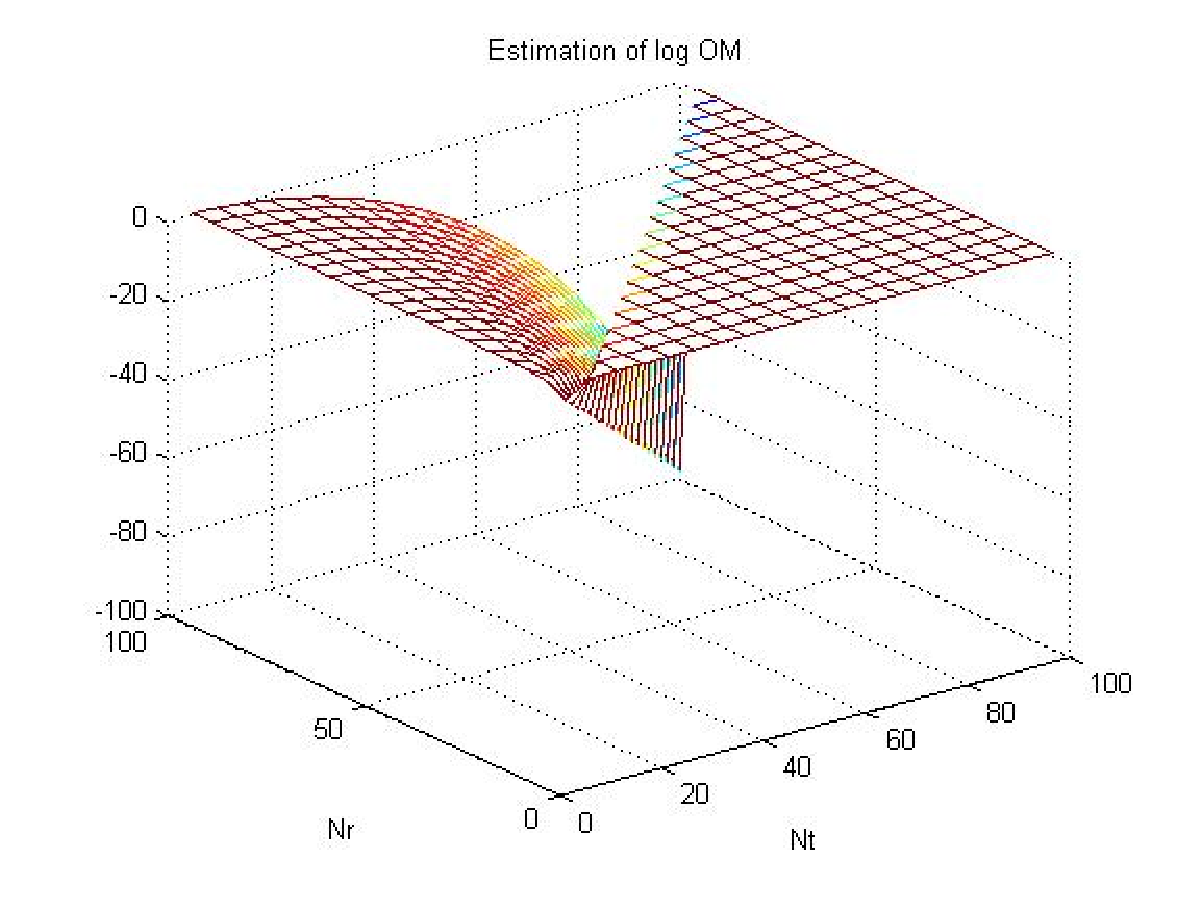
\includegraphics[width=0.7\textwidth, height=5cm]{logE_om_em.eps}
%\caption{Empirical Estimation $E[\ln(\phi_{om})]_{em}$}
%\label{figure1}
%\end{figure}

%\begin{figure}[htb]
%\centering
%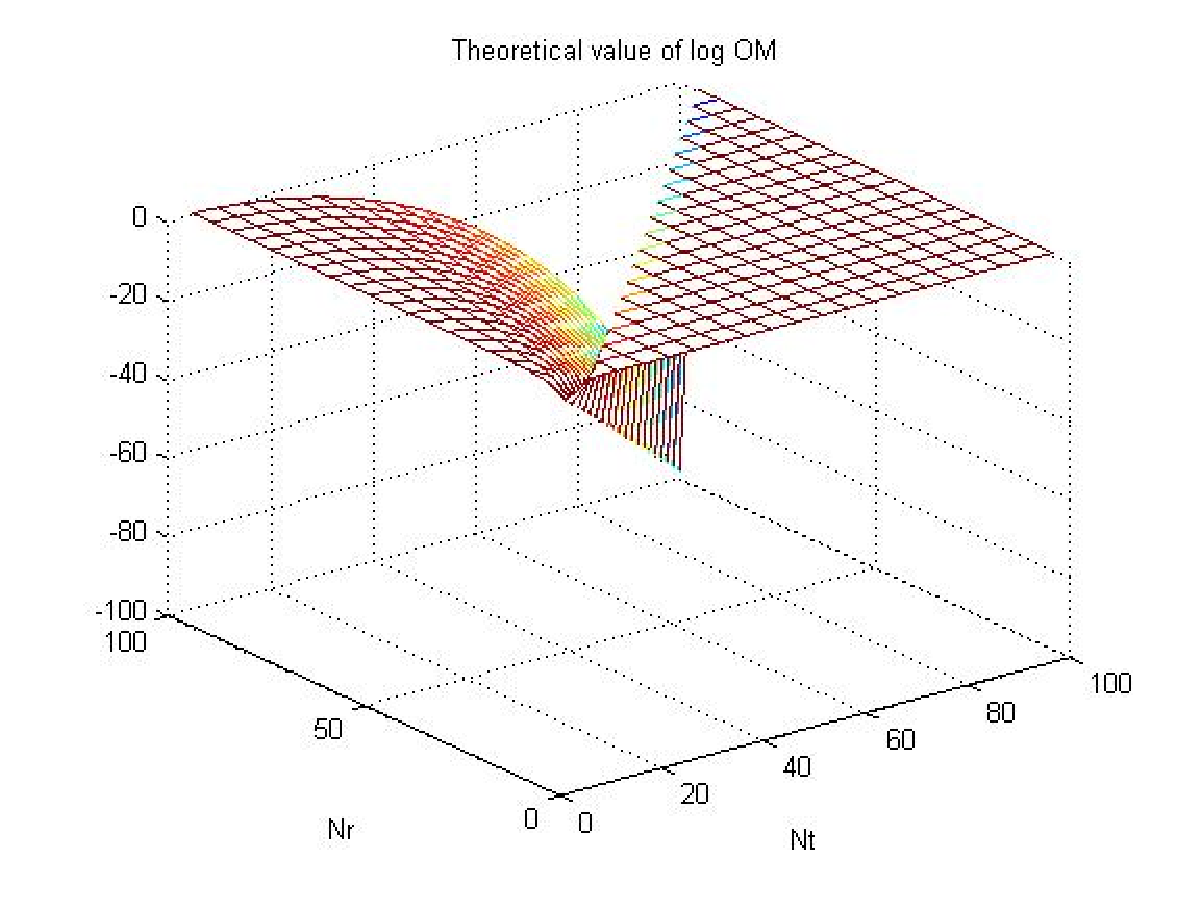
\includegraphics[width=0.7\textwidth, height=5cm]{logE_om_t.eps}
%\caption{Theoretical $E[\ln(\phi_{om})]_{t}$}
%\label{figure2}
%\end{figure} 


%\begin{figure}[htb]
%\centering
%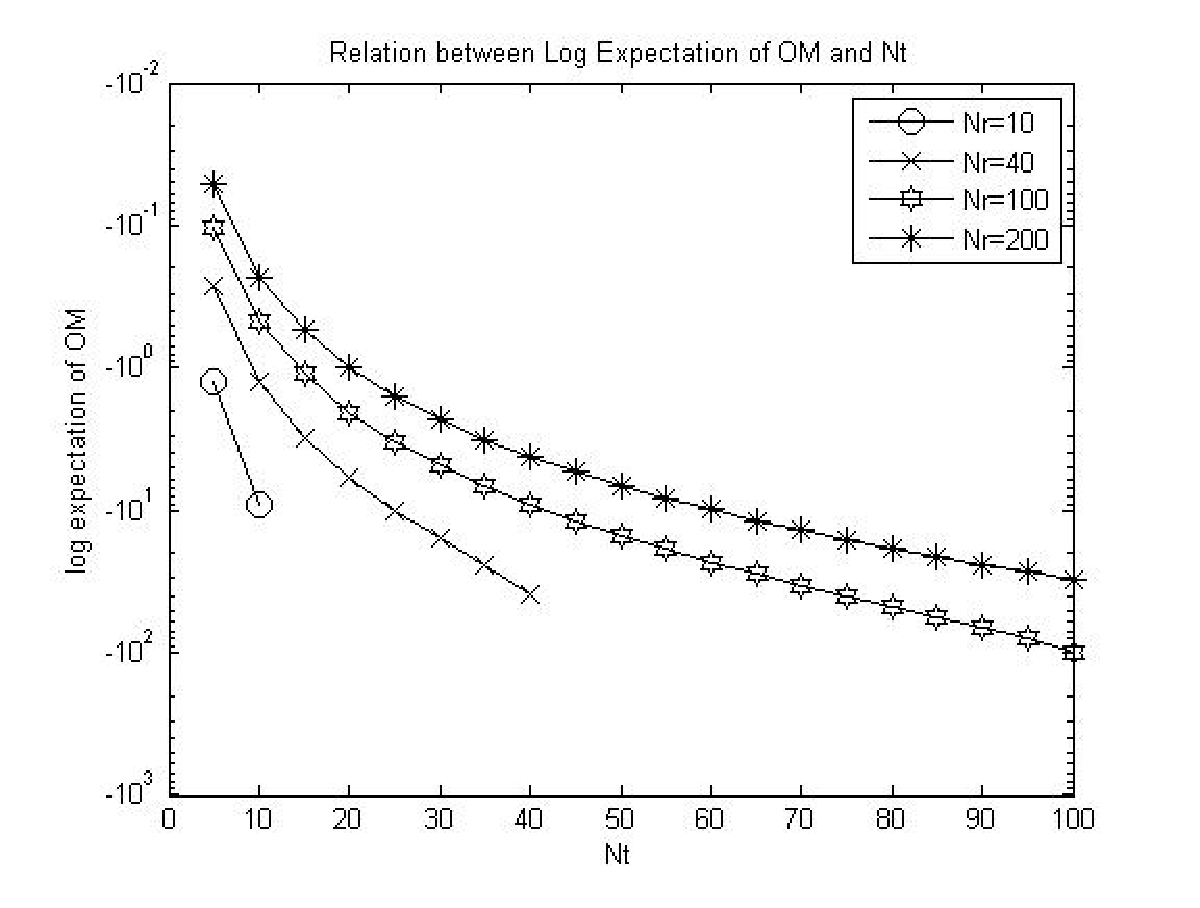
\includegraphics[scale=0.6]{NtE.eps}
%\caption{Relation between $N_{t}$ and $E[\ln(\phi_{om})]_{t}$}
%\label{figure3}
%\end{figure}


\section{Stopping Criteria}\label{stopping criteria}
As discussed in section\ref{section lagrange duality}, in dual objective function, the complementary KKT conditions are the measurement of the proximity of current solution to the optimal solution. 
The feasibility gap, which is a effective stopping criteria used in SVR and SVM, can implicitly monitor whether the KKT complementary conditions are satisfied. The feasibility gap measures the gap between the values of primal objective function and dual objective function. To elaborate a little further, recall the saddle point conditions in section\ref{section lagrange duality}
 \begin{equation}
 L(\mathbf{w}, \bar{\mathbf{a}})\geq L(\bar{\mathbf{w}}, \bar{\mathbf{a}})\geq L(\bar{\mathbf{w}}, \mathbf{a})
 \label{saddle point conditions}
 \end{equation}
Where $(\bar{\mathbf{w}}, \bar{\mathbf{a}})$ are the solution to primal objective function, the KKT complementary conditions are satisfied, that is 
\begin{equation}
\bar{\alpha}_{i}c_{i}(\bar{\mathbf{w}})=0,
\label{complementary KKT condition revisited}
\end{equation}
we have 
\begin{equation}
L(\bar{\mathbf{w}}, \bar{\mathbf{a}})=f(\bar{\mathbf{w}})+\sum_{i=1}^{N_{r}}\bar{\alpha}_{i}c_{i}(\bar{\mathbf{w}})=f(\bar{\mathbf{w}})
\end{equation} 
Let $(\tilde{\mathbf{w}}, \tilde{\mathbf{a}})$ denote the variable pair that satisfies the first and second KKT conditions in (\ref{original KKT condition1} ) and (\ref{original KKT condition2})

\begin{IEEEeqnarray}[\relax]{l}
\label{original KKT condition revisited1}
\partial_{\mathbf{w}}L(\tilde{\mathbf{w}}, \tilde{\mathbf{a}})=\partial_{\mathbf{w}}f(\tilde{\mathbf{w}})+\sum_{i=1}^{L}\tilde{a}_{i}\partial_{\mathbf{w}}c_{i}(\tilde{\mathbf{w}})=0,\\
\label{original KKT condition revisited2}
c_{i}(\tilde{\mathbf{w}})\leq 0, i=1,2,\ldots L
\end{IEEEeqnarray}
based on (\ref{original KKT condition revisited1}), we have 
\begin{IEEEeqnarray}[\relax]{l}
L(\tilde{\mathbf{w}}, \tilde{\mathbf{a}})=f(\tilde{\mathbf{w}})+\sum_{i=1}^{L}\tilde{\alpha}_{i}c_{i}(\tilde{\mathbf{w}})\leq f(\tilde{\mathbf{w}}),
\end{IEEEeqnarray} 
based on Theorem 6.27\cite{scholkopf2002learning}, the following equalities hold
\begin{IEEEeqnarray}[\relax]{l}
f(\tilde{\mathbf{w}})\geq f(\bar{\mathbf{w}})=L(\bar{\mathbf{w}}, \bar{\mathbf{a}})\geq L(\tilde{\mathbf{w}}, \tilde{\mathbf{a}})=f(\tilde{\mathbf{w}})+\sum_{i=1}^{L}\tilde{\alpha}_{i}c_{i}(\tilde{\mathbf{w}})
\label{inequality gap}
\end{IEEEeqnarray}
Therefore the feasibility gap is defined by the gap between the primal objective function $f(\tilde{\mathbf{w}})$ and the dual objective function $L(\tilde{\mathbf{w}}, \tilde{\mathbf{a}})$   
\begin{equation}
f(\tilde{\mathbf{w}})-L(\tilde{\mathbf{w}}, \tilde{\mathbf{a}})=-\sum_{i=1}^{L}\tilde{\alpha}_{i}c_{i}(\tilde{\mathbf{w}})\geq 0
\label{original feasibility gap}
\end{equation}
If the feasibility gap is vanished, based on (\ref{inequality gap}), we have $f(\bar{\mathbf{w}})=f(\tilde{\mathbf{w}})$, thus $\tilde{\mathbf{w}}=\bar{\mathbf{w}}$, $\tilde{\mathbf{a}}=\bar{\mathbf{a}}$. Furthermore, because $f(\tilde{\mathbf{w}})-L(\tilde{\mathbf{w}}, \tilde{\mathbf{a}})=-\sum_{i=1}^{L}\tilde{\alpha}_{i}c_{i}(\tilde{\mathbf{w}})$, the vanish of feasibility gap indicates $\sum_{i=1}^{L}\tilde{\mathbf{a}}c_{i}(\tilde{\mathbf{w}})=0$. Because $\tilde{\alpha}_{i}c_{i}(\tilde{\mathbf{w}})\leq 0, i=1,2,\ldots, L$, we have $\tilde{\alpha}_{i}c_{i}(\tilde{\mathbf{w}})=0, i=1,2,\ldots, L$, the KKT complementary conditions are satisfied. 

In CSVR detector for the large MIMO systems, the primal objective function is
\begin{equation}
f(\tilde{\mathbf{w}}, \xi^{r}_{i}, \hat{\xi}^{r}_{i}, \xi^{i}_{i}, \hat{\xi}_{i}^{i})=\frac{1}{2}||\tilde{\mathbf{w}}||^{2}_{\mathbb{H}}+C\sum_{i=1}^{N_{r}}[R(\xi^{r}_{i})+R(\hat{\xi}^{r}_{i})+R(\xi^{i}_{i})+R(\hat{\xi}^{i}_{i})],
\label{simple primal inter}
\end{equation}
where $\tilde{\mathbf{w}}$ satisfies the KKT  conditions in (\ref{original KKT condition revisited1}) and (\ref{original KKT condition revisited2}).
Define $\lambda^{r}=\alpha-\hat{\alpha}$, $|\lambda^{r}|=\alpha+\hat{\alpha}$ and $\lambda^{i}=\beta-\hat{\beta}$, $|\lambda^{i}|=\beta+\hat{\beta}$, $\Lambda^{r}=[\lambda^{r}_{1}, \lambda^{r}_{2}, \ldots, \lambda^{r}_{L}]^{T}$ and $\Lambda^{i}=[\lambda^{i}_{1}, \lambda_{2}^{i}, \ldots, \lambda^{i}_{L}]^{T}$,
(\ref{complex duality regularization1}) can be rewritten as 
\begin{IEEEeqnarray}[\relax]{l}
||\tilde{\mathbf{w}}||^{2}_{\mathbb{H}}=<(\Lambda^{r})^{T}, \Re{(\mathbf{K})}\Lambda^{r}>+<(\Lambda^{i})^{T}, \Re{(\mathbf{K})}\Lambda^{i}>-2<\Lambda^{r}, \Im{(\mathbf{K})}\Lambda^{i}>,
\label{simple regularization}
\end{IEEEeqnarray}
Therefore we obtain  
\begin{IEEEeqnarray}[\relax]{l}
\nonumber
f(\tilde{\mathbf{w}}, \xi^{r}_{i}, \hat{\xi}^{r}_{i}, \xi^{i}_{i}, \hat{\xi}_{i}^{i})=\frac{1}{2}<(\Lambda^{r})^{T}, \Re{(\mathbf{K})}\Lambda^{r}>+\frac{1}{2}<(\Lambda^{i})^{T}, \Re{(\mathbf{K})}\Lambda^{i}>-<\Lambda^{r}, \Im{(\mathbf{K})}\Lambda^{i}>+C\sum_{i=1}^{N_{r}}[R(\xi^{r}_{i})+\\R(\hat{\xi}^{r}_{i})+R(\xi^{i}_{i})+R(\hat{\xi}^{i}_{i})],
\label{simple primal}
\end{IEEEeqnarray}
Based on (\ref{final complex lagrange duality}), the dual objective function can be rewritten as 
\begin{IEEEeqnarray}[\relax]{l}
\nonumber
\theta(\Lambda^{r}, \Lambda^{i})=-\frac{1}{2}<(\Lambda^{r})^{T}, \Re{(\mathbf{K})}\Lambda^{r}>-\frac{1}{2}<(\Lambda^{i})^{T}, \Re{(\mathbf{K})}\Lambda^{i}>+<\Re(\mathbf{y})^{T}, \Lambda^{r}>+<\Im{(\mathbf{y})}^{T}, \Lambda^{i}>\\
-\epsilon<\mathbf{e}^{T}, (|\Lambda^{r}|+|\Lambda^{i}|)>+C\sum_{i=1}^{N_{r}}[\tilde{R}(\xi^{r}_{i})+\tilde{R}(\hat{\xi}^{r}_{i})+\tilde{R}(\xi^{i}_{i})+\tilde{R}(\hat{\xi}^{i}_{i})],
\label{simple dual function}
\end{IEEEeqnarray}

Based on (\ref{simple primal}) and (\ref{simple dual function}), the feasibility gap is obtained 
\begin{IEEEeqnarray}[\relax]{l}
\nonumber
G(\lambda^{r}, \lambda^{i})=f(\tilde{\mathbf{w}}, \xi^{r}_{i}, \hat{\xi}^{r}_{i}, \xi^{i}_{i}, \hat{\xi}_{i}^{i})-\theta(\Lambda^{r},\Lambda^{i})=<(\Lambda^{r})^{T}, \Re{(\mathbf{K})}\Lambda^{r}>+<(\Lambda^{i})^{T}, \Re{(\mathbf{K})}\Lambda^{i}>-<\Re{(\mathbf{y}^{T})}, \Lambda^{r}>\\\nonumber
-<\Im{(\mathbf{y})}^{T}, \Lambda^{i}>+\epsilon<\mathbf{e}^{T}, (|\Lambda^{r}|+|\Lambda^{i}|)>+C\sum_{i=1}^{N_{r}}[\xi^{r}_{i}R^{'}(\xi^{r}_{i})+\hat{\xi}^{r}_{i}R^{'}(\hat{\xi}^{r}_{i})+\xi^{i}_{i}R^{'}(\xi^{i}_{i})+\hat{\xi}^{i}_{i}R^{'}(\hat{\xi}^{i}_{i})]-\\<\Lambda^{r}, \Im{(\mathbf{K})}\Lambda^{i}>.
\label{simple duality gap}
\end{IEEEeqnarray}
As we explained in section \ref{cost function}, the choice of risk function is determined by distribution of noise, as to Gaussian noise, the risk function is 
\begin{equation}
R(u)=\frac{1}{2}u^{2},
\label{risk function1}
\end{equation} 
hence 
\begin{equation}
\tilde{R}(u)=R(u)-u R{'}(u)=-\frac{1}{2}u^{2},
\label{risk function2}
\end{equation}
In $\epsilon$-SVR, the objective to exploit slack variables is to compensate the influences from the outliers that exceed the $\epsilon$-tube which are caused by the noise.
Therefore in $\epsilon$-SVR, $\xi^{r}_{i}$ and $\hat{\xi}^{r}$ are defined as  
\begin{IEEEeqnarray}[\relax]{l}
\xi^{r}_{i}=\max(0, \Re{(\mathbf{y}_{i})}-\Re{(<\mathbf{h}_{i}, \mathbf{w}>_{\mathbb{H}})}-\epsilon)\\
\hat{\xi}^{r}_{i}=\max(0, \Re{(<\mathbf{h}_{i}, \mathbf{w}>_{\mathbb{H}})}-\Re{(\mathbf{y}_{i})}-\epsilon)
\label{outlier2}
\end{IEEEeqnarray} 
Because the distance between the estimations $\Re{(<\mathbf{h}_{i},\mathbf{w}>_{\mathbb{H}})}$ and the observations $\Re{(\mathbf{y}_{i})}$ can only exceeds the $\epsilon$-tube in one direction, therefore there is at most one of $\xi^{r}_{i}$ and $\hat{\xi}^{r}_{i}$ can be non zero that is $\xi_{i}^{r}\hat{\xi}_{i}^{r}=0$.
Therefore the risk function can be rewritten as 
\begin{IEEEeqnarray}[\relax]{l}
\label{simple risk function1}
R(\xi_{i}^{r})+R(\hat{\xi}_{i}^{r})=\frac{1}{2}|\Re(\mathbf{y}_{i})-\Re(<\mathbf{h}_{i}, \mathbf{w}>_{\mathbb{H}})|_{\epsilon}^{2}\\\label{simple risk function2}
R(\xi_{i}^{i})+R(\hat{\xi}_{i}^{i})=\frac{1}{2}|\Im(\mathbf{y}_{i})-\Im(<\mathbf{h}_{i}, \mathbf{w}>_{\mathbb{H}})|^{2}_{\epsilon}
\end{IEEEeqnarray}
where $|\cdot|_{\epsilon}$ denotes $\epsilon$ insensitive function as mentioned in section \ref{cost function}. Recall (\ref{complex duality regression function}),
\begin{IEEEeqnarray}[\relax]{l}
<\mathbf{h}_{i}, \mathbf{w}>_{\mathbb{H}}
=\sum_{j=1}^{N_{r}}\lambda_{j}^{r}\Re{(\mathbf{K})}_{ij}-\sum_{j=1}^{N_{r}}\lambda^{i}_{j}\Im{(\mathbf{K})}_{ij}+i(\sum_{j=1}^{N_{r}}\lambda_{j}^{r}\Im{(\mathbf{K})}_{ij}+\sum_{j=1}^{N_{r}}\lambda^{i}_{j}\Re{(\mathbf{K})}_{ij}),
\end{IEEEeqnarray}
 we obtain 
\begin{IEEEeqnarray}[\relax]{l}
\label{intermediate function1a}
\Re(\mathbf{y}_{i})-\Re(<\mathbf{h}_{i}, \mathbf{W}>_{\mathbb{H}})=\Re(\mathbf{y}_{i})-\sum_{j=1}^{N_{r}}\lambda^{r}_{j}\Re(\mathbf{K})_{ij}+\sum_{j=1}^{N_{r}}\lambda^{i}_{j}\Im(\mathbf{K})_{ij}\\
\label{intermediate function1b}
\Im(\mathbf{y}_{i})-\Im(<\mathbf{h}_{i}, \mathbf{w}>_{\mathbb{H}})=\Im(\mathbf{y}_{i})-\sum_{j=1}^{N_{r}}\lambda^{i}_{j}\Re(\mathbf{K})_{ij}-\sum_{j=1}^{N_{r}}\lambda^{r}_{j}\Im(\mathbf{K})_{ij}
\end{IEEEeqnarray}
Two intermediate variables $\Phi$ and $\Psi$ are defined
\begin{IEEEeqnarray}[\relax]{l}
\label{intermedia function 2a}
\Phi^{r}=\Re(\mathbf{y})-\Re(\mathbf{K})
\lambda^{r};
\Phi^{i}=\Im(\mathbf{y})-\Re(\mathbf{K})\lambda^{i}\\
\label{intermediate function 2b}
\Psi^{r}=\Im(\mathbf{K})\lambda^{i};
\Psi^{i}=-\Im(\mathbf{K})\lambda^{r}\\
\nonumber
\end{IEEEeqnarray} 
therefore (\ref{intermediate function1a}) and (\ref{intermediate function1b}) can be rewritten as
\begin{IEEEeqnarray}[\relax]{l}
\label{intermediate function3a}
\Re(\mathbf{y}_{i})-\Re(<\mathbf{h}_{i}, \mathbf{W}>_{\mathbb{H}})=\Phi^{r}_{i}+\Psi_{i}^{r}\\\label{intermediate function3b}
\Im(\mathbf{y}_{i})-\Im(<\mathbf{h}_{i}, \mathbf{w}>_{\mathbb{H}})=\Phi_{i}^{i}+\Psi_{i}^{i}
\end{IEEEeqnarray}
Therefore based on (\ref{intermediate function3a}) and (\ref{intermediate function3b}), 
(\ref{simple risk function1}) and (\ref{simple risk function2}) can be rewritten as 
\begin{IEEEeqnarray}[\relax]{l}
\label{intermediate function4a}
R(\xi^{r}_{i})+R(\hat{\xi}^{r}_{i})=\frac{1}{2}|\Phi^{r}_{i}+\Psi_{i}^{r}|^{2}_{\epsilon}\\
\label{intermediate function4b}
R(\xi^{i}_{i})+R(\hat{\xi}^{i}_{i})=\frac{1}{2}|\Phi^{i}_{i}+\Psi_{i}^{i}|^{2}_{\epsilon}
\end{IEEEeqnarray}
Thus based on (\ref{intermediate function4a}) and (\ref{intermediate function4b}), the feasibility gap in (\ref{simple duality gap}) can be rewritten as 
\begin{IEEEeqnarray}[\relax]{l}
\nonumber
G(\Lambda^{r}, \Lambda^{i})=<(\Lambda^{r})^{T}, \Re(\mathbf{K})\Lambda^{r}>+<(\Lambda^{i})^{T}, \Re(\mathbf{K})\Lambda^{i}>-<\Re(\mathbf{y})^{T}, \Lambda^{r}>-<\Im(\mathbf{y})^{T}, \Lambda^{i}>\\
+\epsilon<\mathbf{e}^{T}, (|\Lambda^{r}|+|\Lambda^{i}|)>+C\sum_{i=1}^{N_{r}}[(|\Phi^{r}_{i}+\Psi^{r}_{i}|)^{2}_{\epsilon}+(|\Phi^{i}_{i}+\Psi^{i}_{i}|)^{2}_{\epsilon}]-<\Lambda^{r}, \Im(\mathbf{K})\Lambda^{i}>.
\label{simple duality gap final}
\end{IEEEeqnarray}
Based on dual objective function in (\ref{simple dual function}), (\ref{simple duality gap final}) can be rewritten as 
\begin{IEEEeqnarray}[\relax]{l}
\nonumber
G(\Lambda^{r}, \Lambda^{i})=<\Re(\mathbf{y})^{T}, \Lambda^{r}>+<\Im(\mathbf{y})^{T}, \Lambda^{i}>-\epsilon<\mathbf{e}^{T}, (|\Lambda^{r}|+|\Lambda^{i}|)>-2\theta(\Lambda_{i}, \Lambda_{j})\\
-<\Lambda^{r}, \Im(\mathbf{K})\Lambda^{i}>.\label{simple duality gap1}
\end{IEEEeqnarray}
The following ratio of the feasibility gap $G(\Lambda^{r}, \Lambda^{i})$ is used to measure the proximity of current solution to the optimal solution. The algorithm stops when the ratio satisfies a certain tolerance.
\begin{equation}
\frac{G}{G+\theta}
\label{simple duality gap ratio1}
\end{equation}
\subsection{Update $\Phi$, $\Psi$ and $G$}
$\Phi$, $\Psi$ and $G$ are updated in each iteration along with the optimization variables updated. The pseudo code to update $\Phi$, $\Psi$ and $G$ is given.

Based on the definitions of $\Phi$ and $\Psi$ in (\ref{intermedia function 2a}) and (\ref{intermediate function 2b}), we have the following procedure to update $\Phi$ and $\Psi$ in real channel and imaginary channel, assume the optimization variables updated in each channel are indexed by $1$ and $2$, let $\sigma^{r}_{i}=(\lambda^{r}_{i})^{new}-\lambda^{r}_{i}$ and $\sigma^{i}_{i}=(\lambda^{i}_{i})^{new}-\lambda^{i}_{i}$ denote the differences between the updated optimization variables and the old optimization variables.\\
\begin{algorithm}[htb]
\begin{algorithmic}
\Procedure{\textbf{1}. Update $\Phi^{r}$ and $\Psi^{i}$ in real channel}{}
\For{$i=1:N_{r}$}
\State $\Phi_{i}^{r}=\Phi_{i}^{r}-\sigma_{1}^{r}\mathbf{K}^{r}_{i1}-\sigma_{2}^{r}\mathbf{K}_{i2}^{r}$
\State $\Psi_{i}^{i}=\Psi_{i}^{i}-\sigma_{1}^{r}\mathbf{K}^{i}_{i1}-\sigma_{2}^{r}\mathbf{K}^{i}_{i2}$
\EndFor
\EndProcedure
\end{algorithmic}
\end{algorithm}
\begin{algorithm}[htb]
\begin{algorithmic}
\Procedure{\textbf{2}. Update $\Phi^{i}$ and $\Psi^{r}$ in imaginary channel}{}
\For{$i=1:N_{r}$}
\State $\Phi_{i}^{i}=\Phi_{i}^{i}-\sigma_{1}^{i}\mathbf{K}^{r}_{i1}-\sigma_{2}^{i}\mathbf{K}_{i2}^{r}$
\State $\Psi_{i}^{r}=\Psi_{i}^{r}+\sigma_{1}^{i}\mathbf{K}^{i}_{i1}+\sigma_{2}^{i}\mathbf{K}^{i}_{i2}$
\EndFor
\EndProcedure
\end{algorithmic}
\end{algorithm}

Then the cost function term in (\ref{simple duality gap final}) are updated by \textbf{Procedure 3} and \textbf{Procedure 4}. The cost function terms are denoted by $\chi^{r}$ in real channel and $\chi^{i}$ in imaginary channel.
\begin{IEEEeqnarray}[\relax]{l}
\label{cost function update1}
\chi^{r}=\sum_{i}^{N_{r}}|\Phi^{r}_{i}+\Psi^{r}_{i}|^{2}_{\epsilon}\\
\label{cost function update2}
\chi^{i}=\sum_{i}^{N_{r}}|\Phi^{i}_{i}+\Psi^{i}_{i}|^{2}_{\epsilon}
\end{IEEEeqnarray}
\begin{algorithm}[htb]
\begin{algorithmic}
\Procedure{\textbf{3}. Update cost function in real channel}{$\chi^{r}$}
\State $\chi^{r}=0$  \Comment{initial risk term}
\For{$i=1:N_{r}$}
\If{$|\Phi^{r}_{i}+\Psi^{r}_{i}|>\epsilon$}
\State $\chi^{r}+=(|\Phi^{r}_{i}+\Psi^{r}_{i}|-\epsilon)^{2}$
\EndIf
\EndFor
\EndProcedure
\end{algorithmic}
\end{algorithm}

\begin{algorithm}[htb]
\begin{algorithmic}
\Procedure{\textbf{4}. Update cost function in imaginary channel}{$\chi^{i}$}
\State $\chi^{i}=0$  \Comment{initial risk term}
\For{$i=1:N_{r}$}
\If{$|\Phi^{i}_{i}+\Psi^{i}_{i}|>\epsilon$}
\State $\chi^{i}+=(|\Phi^{i}_{i}+\Psi^{i}_{i}|-\epsilon)^{2}$
\EndIf
\EndFor
\EndProcedure
\end{algorithmic}
\end{algorithm}
The pseudo code to update duality gap $G$ based on (\ref{simple duality gap1}) is shown in \textbf{Procedure 5}. Assume the indexes of optimization variables updated in real channel is $i$ and $j$, the indexes of optimization variables updated in imaginary channel is $m$ and $f$. Define the work sets in real and imaginary channels $S^{r}=[i,j]$ and $S^{i}=[m,f]$. Define $(\chi^{r})^{new}$ and $(\chi^{i})^{new}$ are the updated cost function terms based on \textbf{Procedure 3} and \textbf{Procedure 4}, the update process for the term $\theta(\Lambda^{r}, \Lambda^{i})$ in (\ref{simple duality gap1}) can be written as 
\begin{equation}
\bigtriangledown \theta(\Lambda^{r}_{S^{r}}, \Lambda^{i}_{S^{i}})=\bigtriangledown \theta^{r}_{S^{r}}+\bigtriangledown \theta^{i}_{S^{i}}-\frac{C}{2}((\chi^{r})^{new}+(\chi^{i})^{new}-\chi^{r}-\chi^{i}),
\label{update dual objective function}
\end{equation}
Where $\theta_{S}^{r}$ is the gain of the sub dual objective function as shown in (\ref{gain work set selection lambda}), 
\begin{IEEEeqnarray}[\relax]{l}
\bigtriangledown \theta_{S^{r}}^{r}=-\frac{1}{2}(\Sigma^{r}_{S^{r}})^{T}\Re{(\mathbf{K})}_{S^{r}S^{r}}\Sigma^{r}_{S^{r}}+(\Phi^{r}_{S^{r}})^{T}\Sigma^{r}_{S^{r}}-\epsilon<\mathbf{e}^{T}_{S^{r}},|(\Lambda^{r}_{S^{r}})^{new}|-|\Lambda^{r}_{S^{r}}|>\\
\bigtriangledown \theta_{S^{i}}^{i}=-\frac{1}{2}(\Sigma^{i}_{S^{i}})^{T}\Re{(\mathbf{K})}_{S^{i}S^{i}}\Sigma^{i}_{S^{i}}+(\Phi^{i}_{S^{i}})^{T}\Sigma^{i}_{S^{i}}-\epsilon<\mathbf{e}^{T}_{S^{i}},|(\Lambda^{i}_{S^{i}})^{new}|-|\Lambda^{i}_{S^{i}}|>
\end{IEEEeqnarray}
\begin{algorithm}[htb]
\begin{algorithmic}
\Procedure{\textbf{5}. Update $G$}{}
\State $G+=Re(\mathbf{y}_{1})\sigma^{r}_{i}+Re(\mathbf{y}_{2})\sigma^{r}_{j}$
\State $G+=Im(\mathbf{y}_{1})\sigma^{i}_{m}+Re(\mathbf{y}_{2})\sigma^{i}_{f}$
\State $G-=\epsilon(|\lambda^{r}_{i}+\sigma^{r}_{i}|-|\lambda^{r}_{i}|+|\lambda^{r}_{j}+\sigma^{r}_{j}|-|\lambda^{r}_{j}|)$
\State $G-=\epsilon(|\lambda^{i}_{m}+\sigma^{i}_{m}|-|\lambda^{i}_{m}|+|\lambda^{i}_{f}+\sigma^{i}_{f}|-|\lambda^{i}_{f}|)$
\State $G-=2(\bigtriangledown \theta(\Lambda^{r}_{S^{r}}, \Lambda^{i}_{S^{i}}))$ \Comment{Update sub objective function based on (\ref{update dual objective function})}

\State $G-=(\Sigma^{r}_{S^{r}})^{T}\Im(\mathbf{K}_{S^{r}S^{i}})\Sigma^{i}_{S^{i}}+(\Sigma^{r}_{S^{r}})^{T}\Psi^{r}_{S^{r}}+(\Sigma^{i}_{S^{i}})^{T}\Psi^{i}_{S^{i}}$ \Comment{Update $<\Lambda^{r},\Im(\mathbf{K})\Lambda^{i}>$}
\EndProcedure
\label{update G Phi and Psi}
\end{algorithmic}
\end{algorithm}


Pseudo code for two types of combined 1-D searching solver are given by \textbf{Procedure 6} and \textbf{Procedure 7}. 
\begin{algorithm}[htb]
\begin{algorithmic}
\Procedure{\textbf{6}. One-shot 1-D combined searching solver}{} 
\State Step 1. Search for two optimization variables based on single direction solver
\For{$i=1:N_{r}$}
\State calculate $\bigtriangledown \theta^{r}_{i}(\bigtriangledown \theta_{i}^{i})$\Comment{Based on single direction solver \ref{single direction solver}}
\EndFor
\State choose the dual variable with first and the second largest gain of sub objective function, denoted as 1st and 2nd
\State Step 2. Update 1st and 2nd optimization variables based on double direction solver 
\State update $\lambda^{r}_{1st}(\lambda^{i}_{1st})$ and $\lambda^{r}_{2nd}(\lambda^{i}_{2nd})$\Comment{Based on double direction solver \ref{double direction solver}}
\State update $\Phi^{r}(\Phi^{i})$ and $\Psi^{r}(\Psi^{i})$ by \textbf{Procedure 1} and \textbf{Procedure 2}
\EndProcedure
\end{algorithmic}
%\caption{Sequential 2-D Solver without Damping}
\label{1D2D Nodamping}
\end{algorithm} 
 
 
 \begin{algorithm}[htb]
\begin{algorithmic}
\Procedure{\textbf{7}. Sequential 1-D combined searching solver}{}
\State Step 1. Search for two optimization variables based on single direction solver
\For{$i=1:N_{r}$}\Comment{First round searching}
\State calculate $\bigtriangledown \theta_{i}^{r}(\bigtriangledown \theta_{i}^{i})$ \Comment{Based on single direction solver \ref{single direction solver}}
\EndFor
\State choose the optimization variable with the largest gain of objective function as $1st_{1}$
\State update $\Phi^{r}(\Phi^{i})$ and $\Psi^{r}(\Psi^{i})$ with respect to $1st_{1}$
\For{$i=1:N_{r}$} \Comment{Second round searching}
\State calculate $\bigtriangledown \theta_{i}^{r}(\bigtriangledown \theta_{i}^{i})$ \Comment{Based on single direction solver \ref{single direction solver}}
\EndFor
\State choose the optimization variable with the largest gain of objective function as $1st_{2}$
\State Step 2. Update $1st_{1}$ and $1st_{2}$ optimization variables based on double direction solver 
\State update $\lambda^{r}_{1st_{1}}(\lambda^{i}_{1st_{1}})$ and $\lambda^{r}_{1st_{2}}(\lambda^{i}_{1st_{2}})$\Comment{Based on double direction solver \ref{double direction solver}}
\State update $\Phi^{r}(\Phi^{i})$ and $\Psi^{r}(\Psi^{i})$ by \textbf{Procedure 1} and \textbf{Procedure 2}

\EndProcedure
\end{algorithmic}
%\caption{Sequential 2-D Solver with Damping}
\label{1D2D damping}
\end{algorithm} 
\newpage
The pseudo code of complex support vector detector (CSVD) is shown in Appendix \ref{Pseudo code of CSVD}


 
%\section{Hyperparameter Setting}
\section{Computer Simulations}
Computer simulations are launched to test the detection and run time performance of proposed dual channel complex support vector detection algorithm. For sake of brevity, the real case is tested first, all the experiments are made by C, compiled by gcc version 4.8.3 on 64 bit Fedora (release 19) Linux system. The experiment platform is a desktop computer with I5-4th generation CPU with quad processing cores, 3.2 GHz clock rate, 8 GB RAM. 

For sake of brevity, we consider a real uncoded spatial multiplex large MIMO system to simulate one channel of the proposed dual channel complex support vector detection algorithm.  with $N_{r}$ received antennas and $N_{t}$ transmitted antennas. The propagation channel matrix is constructed by channel gain components that are identically independent distributed (i.i.d) Gaussian random variables with zero mean and unit variance. transmitted symbols are mutually independent modulated by $M$ PAM with normalized average energy $\frac{1}{N_{t}}$, transmitted over flat fading channel, the sample of noise is AWGN with zero mean and variance $\frac{1}{10^{SNR/10}}$, where $SNR$ denotes the signal to noise ratio. 
We make experiment to low loading factor system $100\times 40$ and full loading factor $100\times 100$, with at least $1e^{5}$ channel realizations and at least $500$ symbol errors accumulated. Fig.\ref{SER performance} shows the symbol error rate (SER) performance, Table.\ref{iteration time} shows the average iteration time of real SVD for different SNR. 
\begin{figure}[htb]
\centering
%\def\svgscale{0.5}
\def\svgwidth{\columnwidth}
\input{BER_curve_real_system.pdf_tex}
\caption{SER performance of $100\times 100 $ and $100\times 40$ MIMO system}
\label{SER performance}
\end{figure}

\begin{table}[htb]
\renewcommand{\arraystretch}{1.3}
\caption{Average Iteration Time of Real Support Vector Detector}
\label{iteration time}
\centering
\begin{tabular}{|c|c|c|c|c|c|c|c|c|c|}
\hline
\multirow{2}{*} {\bfseries Array Size} & \multicolumn{9}{|c|}{\bfseries SNR}\\
\cline{2-10}
 &6& 8 &10& 12& 14& 16& 18& 20& 22\\
\hline
$100\times 40$&682 &681 &681 &681& 680 &679 &678&677 & 680\\
\hline
$100\times 100$&1925 &1916& 1903& 1885& 1862& 1827& 1782&1723&1654 \\
\hline
\end{tabular}
\end{table}
% An example of a floating figure using the graphicx package.
% Note that \label must occur AFTER (or within) \caption.
% For figures, \caption should occur after the \includegraphics.
% Note that IEEEtran v1.7 and later has special internal code that
% is designed to preserve the operation of \label within \caption
% even when the captionsoff option is in effect. However, because
% of issues like this, it may be the safest practice to put all your
% \label just after \caption rather than within \caption{}.
%
% Reminder: the "draftcls" or "draftclsnofoot", not "draft", class
% option should be used if it is desired that the figures are to be
% displayed while in draft mode.
%
%\begin{figure}[!t]
%\centering
%\includegraphics[width=2.5in]{myfigure}
% where an .eps filename suffix will be assumed under latex, 
% and a .pdf suffix will be assumed for pdflatex; or what has been declared
% via \DeclareGraphicsExtensions.
%\caption{Simulation results for the network.}
%\label{fig_sim}
%\end{figure}

% Note that IEEE typically puts floats only at the top, even when this
% results in a large percentage of a column being occupied by floats.


% An example of a double column floating figure using two subfigures.
% (The subfig.sty package must be loaded for this to work.)
% The subfigure \label commands are set within each subfloat command,
% and the \label for the overall figure must come after \caption.
% \hfil is used as a separator to get equal spacing.
% Watch out that the combined width of all the subfigures on a 
% line do not exceed the text width or a line break will occur.
%
%\begin{figure*}[!t]
%\centering
%\subfloat[Case I]{\includegraphics[width=2.5in]{box}%
%\label{fig_first_case}}
%\hfil
%\subfloat[Case II]{\includegraphics[width=2.5in]{box}%
%\label{fig_second_case}}
%\caption{Simulation results for the network.}
%\label{fig_sim}
%\end{figure*}
%
% Note that often IEEE papers with subfigures do not employ subfigure
% captions (using the optional argument to \subfloat[]), but instead will
% reference/describe all of them (a), (b), etc., within the main caption.
% Be aware that for subfig.sty to generate the (a), (b), etc., subfigure
% labels, the optional argument to \subfloat must be present. If a
% subcaption is not desired, just leave its contents blank,
% e.g., \subfloat[].


% An example of a floating table. Note that, for IEEE style tables, the
% \caption command should come BEFORE the table and, given that table
% captions serve much like titles, are usually capitalized except for words
% such as a, an, and, as, at, but, by, for, in, nor, of, on, or, the, to
% and up, which are usually not capitalized unless they are the first or
% last word of the caption. Table text will default to \footnotesize as
% IEEE normally uses this smaller font for tables.
% The \label must come after \caption as always.
%
%\begin{table}[!t]
%% increase table row spacing, adjust to taste
%\renewcommand{\arraystretch}{1.3}
% if using array.sty, it might be a good idea to tweak the value of
% \extrarowheight as needed to properly center the text within the cells
%\caption{An Example of a Table}
%\label{table_example}
%\centering
%% Some packages, such as MDW tools, offer better commands for making tables
%% than the plain LaTeX2e tabular which is used here.
%\begin{tabular}{|c||c|}
%\hline
%One & Two\\
%\hline
%Three & Four\\
%\hline
%\end{tabular}
%\end{table}


% Note that the IEEE does not put floats in the very first column
% - or typically anywhere on the first page for that matter. Also,
% in-text middle ("here") positioning is typically not used, but it
% is allowed and encouraged for Computer Society conferences (but
% not Computer Society journals). Most IEEE journals/conferences use
% top floats exclusively. 
% Note that, LaTeX2e, unlike IEEE journals/conferences, places
% footnotes above bottom floats. This can be corrected via the
% \fnbelowfloat command of the stfloats package.
%\section{Complexity Analysis}


%\section{Conclusion}
%The conclusion goes here.





% if have a single appendix:
%\appendix[Proof of the Zonklar Equations]
% or
%\appendix  % for no appendix heading
% do not use \section anymore after \appendix, only \section*
% is possibly needed

% use appendices with more than one appendix
% then use \section to start each appendix
% you must declare a \section before using any
% \subsection or using \label (\appendices by itself
% starts a section numbered zero.)
%

\appendices
%\section{Proof of the First Zonklar Equation}
%Appendix one text goes here.

% you can choose not to have a title for an appendix
% if you want by leaving the argument blank
\section{Pseudo Code of CSVD}\label{Pseudo code of CSVD}
\begin{algorithm}[htb]
\begin{algorithmic}
\Procedure{CSVD}{$\mathbf{y}$,$\mathbf{H}$}
\State Step 1. Initialization
\State $\mathbf{K}=\mathbf{H}\mathbf{H}^{H}$ \Comment{kernel matrix}
\State $\chi^{r}=0$, $\chi^{i}=0$ \Comment{risk function}
\For{$i=1:N_{r}$}\Comment{initialize $\lambda^{r}$, $\lambda^{i}$, $\Phi^{r}$, $\Phi^{i}$, $\Psi^{r}$, $\Psi^{i}$ and duality gap $G$}
\State $\lambda_{i}^{r}=0, \lambda_{i}^{i}=0$
\State $\Phi_{i}^{r}=Re(y_{i}), \Phi_{i}^{i}=Im(y_{i})$
\State $\Psi_{i}^{r}=0, \Psi_{i}^{i}=0$
\If{$|\Phi^{r}_{i}|>\epsilon$}
\State $\chi^{r}+=(|\Phi^{r}_{i}|-\epsilon)^{2}$
\EndIf
\If{$|\Phi^{i}_{i}|>\epsilon$}
\State $\chi^{i}+=(|\Phi_{i}^{i}|-\epsilon)^{2}$
\EndIf
\EndFor 
\State $G=C(\chi^{r}+\chi^{i})$ \Comment{initialize duality gap}
\State $\theta=-0.5G$ \Comment{initialize objective function}
\State  Step 2. if $G>tol$, go to step 3, else go to Step 5
\State Step 3.
\State call combined 1-D searching solver in \textbf{Procedure 6} and \textbf{Procedure 7} \Comment{find and update two optimization variables in the real and imaginary channel} 
\State Step 4. \textbf{Procedure 5} update $\frac{G}{G+\theta}$, go back to step 2.
\State Step 5.
\State $\tilde{\mathbf{x}}=\mathbf{H}^{H}(\Lambda^{r}+i\Lambda^{i})$ \Comment{reconstruct $\mathbf{x}$}
\State $\mathbf{x}=\mathbb{Q}(\tilde{x})$\Comment{$\mathbb{Q}(\cdot)$ denotes quantization operation based on symbol constellation}
\State Step 6. \textbf{Return} $\mathbf{x}$ 
\EndProcedure
\end{algorithmic}
\label{CSVD algorithm}
\caption{Dual Channel Complex Support Vector Detection Algorithm }
\end{algorithm}
%Appendix two text goes here.


% use section* for acknowledgment
%\section*{Acknowledgment}


%The authors would like to thank...


% Can use something like this to put references on a page
% by themselves when using endfloat and the captionsoff option.
%\ifCLASSOPTIONcaptionsoff
%  \newpage
%\fi



% trigger a \newpage just before the given reference
% number - used to balance the columns on the last page
% adjust value as needed - may need to be readjusted if
% the document is modified later
%\IEEEtriggeratref{8}
% The "triggered" command can be changed if desired:
%\IEEEtriggercmd{\enlargethispage{-5in}}

% references section

% can use a bibliography generated by BibTeX as a .bbl file
% BibTeX documentation can be easily obtained at:
% http://www.ctan.org/tex-archive/biblio/bibtex/contrib/doc/
% The IEEEtran BibTeX style support page is at:
% http://www.michaelshell.org/tex/ieeetran/bibtex/
%\bibliographystyle{IEEEtran}
% argument is your BibTeX string definitions and bibliography database(s)
%\bibliography{IEEEabrv,../bib/paper}
%
% <OR> manually copy in the resultant .bbl file
% set second argument of \begin to the number of references
% (used to reserve space for the reference number labels box)
%\begin{thebibliography}{1}

%\bibitem{IEEEhowto:kopka}
%H.~Kopka and P.~W. Daly, \emph{A Guide to \LaTeX}, 3rd~ed.\hskip 1em plus
%  0.5em minus 0.4em\relax Harlow, England: Addison-Wesley, 1999.

%\end{thebibliography}

% biography section
% 
% If you have an EPS/PDF photo (graphicx package needed) extra braces are
% needed around the contents of the optional argument to biography to prevent
% the LaTeX parser from getting confused when it sees the complicated
% \includegraphics command within an optional argument. (You could create
% your own custom macro containing the \includegraphics command to make things
% simpler here.)
%\begin{IEEEbiography}[{\includegraphics[width=1in,height=1.25in,clip,keepaspectratio]{mshell}}]{Michael Shell}
% or if you just want to reserve a space for a photo:

%\begin{IEEEbiography}{Michael Shell}
%Biography text here.
%\end{IEEEbiography}

% if you will not have a photo at all:
%\begin{IEEEbiographynophoto}{John Doe}
%Biography text here.
%\end{IEEEbiographynophoto}

% insert where needed to balance the two columns on the last page with
% biographies
%\newpage

%\begin{IEEEbiographynophoto}{Jane Doe}
%Biography text here.
%\end{IEEEbiographynophoto}

% You can push biographies down or up by placing
% a \vfill before or after them. The appropriate
% use of \vfill depends on what kind of text is
% on the last page and whether or not the columns
% are being equalized.

%\vfill

% Can be used to pull up biographies so that the bottom of the last one
% is flush with the other column.
%\enlargethispage{-5in}



% that's all folks
%\end{spacing}

\newpage
\bibliographystyle{IEEEtran}
\bibliography{citation}	
\end{spacing}												
\end{document}




